% vim: set tw=80:spell
%
\documentclass[twoside,a5paper,10pt]{extarticle}
%\documentclass[twoside,14pt,draft]{extarticle}
%\documentclass[twoside,14pt,draft]{scrartcl}
\usepackage{amsmath}
\usepackage{amssymb}
\usepackage{amsfonts}
\usepackage{mathtext}
\usepackage{pdfpages}
\usepackage{parallel}
\usepackage[T2A]{fontenc}
\usepackage{ucs}
\usepackage[utf8x]{inputenc}
\usepackage[polish,english,russian]{babel}
\usepackage{hyperref}
\usepackage{rotating}
\usepackage[inner=2cm,top=1.8cm,outer=2cm,bottom=2.3cm,nohead]{geometry}
\usepackage{listings}
\usepackage{graphicx}
\usepackage{wrapfig}
\usepackage{longtable}
\usepackage{indentfirst}
\usepackage{array}
\newcolumntype{P}[1]{>{\raggedright\arraybackslash}p{#1}}
\frenchspacing
\usepackage{fixltx2e} %text sub- and superscripts
\usepackage{icomma} % коскі ў матэматычным рэжыме
\PreloadUnicodePage{4}

\newcommand{\longpage}{\enlargethispage{\baselineskip}}
\newcommand{\shortpage}{\enlargethispage{-\baselineskip}}

\def\switchlang#1{\expandafter\csname switchlang#1\endcsname}
\def\switchlangbe{
\let\saverefname=\refname%
\def\refname{Літаратура}%
\def\figurename{Іл.}%
}
\def\switchlangen{
\let\saverefname=\refname%
\def\refname{References}%
\def\figurename{Fig.}%
}
\def\switchlangru{
\let\saverefname=\refname%
\let\savefigurename=\figurename%
\def\refname{Литература}%
\def\figurename{Рис.}%
}

\hyphenation{admi-ni-stra-tive}
\hyphenation{ex-pe-ri-ence}
\hyphenation{fle-xi-bi-li-ty}
\hyphenation{Py-thon}
\hyphenation{ma-the-ma-ti-cal}
\hyphenation{re-ported}
\hyphenation{imp-le-menta-tions}
\hyphenation{pro-vides}
\hyphenation{en-gi-neering}
\hyphenation{com-pa-ti-bi-li-ty}
\hyphenation{im-pos-sible}
\hyphenation{desk-top}
\hyphenation{elec-tro-nic}
\hyphenation{com-pa-ny}
\hyphenation{de-ve-lop-ment}
\hyphenation{de-ve-loping}
\hyphenation{de-ve-lop}
\hyphenation{da-ta-ba-se}
\hyphenation{plat-forms}
\hyphenation{or-ga-ni-za-tion}
\hyphenation{pro-gramming}
\hyphenation{in-stru-ments}
\hyphenation{Li-nux}
\hyphenation{sour-ce}
\hyphenation{en-vi-ron-ment}
\hyphenation{Te-le-pathy}
\hyphenation{Li-nux-ov-ka}
\hyphenation{Open-BSD}
\hyphenation{Free-BSD}
\hyphenation{men-ti-on-ed}
\hyphenation{app-li-ca-tion}

\def\progref!#1!{\texttt{#1}}
\renewcommand{\arraystretch}{2} %Іначай формулы ў матрыцы зліпаюцца з лініямі
\usepackage{array}

\def\interview #1 (#2), #3, #4, #5\par{

\section[#1, #3, #4]{#1 -- #3, #4}
\def\qname{LVEE}
\def\aname{#1}
\def\q ##1\par{{\noindent \bf \qname: ##1 }\par}
\def\a{{\noindent \bf \aname: } \def\qname{L}\def\aname{#2}}
}

\def\interview* #1 (#2), #3, #4, #5\par{

\section*{#1\\{\small\rm #3, #4. #5}}

\def\qname{LVEE}
\def\aname{#1}
\def\q ##1\par{{\noindent \bf \qname: ##1 }\par}
\def\a{{\noindent \bf \aname: } \def\qname{L}\def\aname{#2}}
}

%\usepackage{portland}
%\usepackage{lscape}
%\usepackage{rotating}
\usepackage[labelsep=period,justification=centering]{caption}
%\usepackage{ccaption}
%\captiondelim{. }
\usepackage{hyphenat}
\usepackage{tweaklist}
\usepackage{pdfpages}
%\usepackage{trace}
%\usepackage{tikz}
%\usetikzlibrary{calc}
%\usetikzlibrary{positioning}
\usepackage{subfig}
\renewcommand{\enumhook}{\setlength{\topsep}{0pt}%
  \setlength{\itemsep}{0pt}\setlength{\parskip}{0pt plus 1pt minus 1pt}\setlength{\parsep}{0pt}}
\renewcommand{\itemhook}{\setlength{\topsep}{0pt}%
  \setlength{\itemsep}{0pt}\setlength{\parskip}{0pt plus 1pt minus 1pt}\setlength{\parsep}{0pt}}
%\renewcommand{\enumhook}{\setlength{\topsep}{0pt}%
%  \setlength{\itemsep}{0pt}}
%\renewcommand{\itemhook}{\setlength{\topsep}{0pt}%
%  \setlength{\itemsep}{0pt}\setlength{\parskip}{0pt}\setlength{\parsep}{0pt}}
%\renewcommand{\enumhook}{\setlength{\topsep}{0pt}%
%  \setlength{\itemsep}{0pt}}
%\renewcommand{\itemhook}{\setlength{\topsep}{0pt}%
%  \setlength{\itemsep}{0pt}\setlength{\parsep}{0pt}}

\clubpenalty=10000%
\widowpenalty=10000%
%\setlength{\parindent}{1.25cm}%

\newcommand\familyname[1]{\textbf{#1}}

\DeclareMathOperator{\e}{e}
\DeclareMathOperator{\cov}{cov}
\DeclareMathOperator{\diag}{diag}

\newcommand\eof{\writetotalpages\end{document}\endinput}

\newcommand\key[1]{\textbf{#1}}
\newcommand\vect[1]{\mathbf{#1}}
\def\eqn #1 $#2${\begin{equation}\label{eq:#1}#2\end{equation}}
%\def\where #1
\newcommand\eqnref[1]{(\ref{eq:#1})}
\makeatletter
\def\p@subfigure{\thefigure,~}
\def\thesubfigure{\asbuk{subfigure}}
\newcounter{articleno}
\setcounter{articleno}0
\@newctr{figure}[articleno]
\renewcommand \thefigure {\@arabic\c@articleno.\@arabic\c@figure}
\@newctr{equation}[articleno]
\renewcommand\theequation{\@arabic\c@articleno.\@arabic\c@equation}
\newcommand\ps@twoside{%
 \makeatletter%
 \renewcommand\@oddfoot{~\hfill\thepage}%
 \renewcommand\@evenfoot{\thepage\hfill~}%
 \makeatother%
}
\newcounter{totalpages}
\def\writetotalpages{%
  \protected@write\@auxout
      {}%
      {\string\setcounter{totalpages}{\thepage}}}
\newcounter{totalfigures}%
\newcounter{totalsubfigures}%
\newcounter{totalsections}%
\newcounter{totalsubsections}%
\newcounter{totalsubsubsections}%
\newcounter{totalparagraphs}%

%\def\addcontentsline#1#2#3{%
%  \addtocontents{#1}{\protect\contentsline{#2}{#3}{\thepage}%
%  \protect\stepcounter{total#2s}}}
\makeatother
\newcommand\comment[1]{\textsf{#1}}
\renewcommand\labelitemi{\textendash}
\renewcommand\labelitemii{\textendash}


% перенос формул в тексте
\newcommand*{\hm}[1]{#1\nobreak\discretionary{}%
  {\hbox{$\mathsurround=0pt #1$}}{}}

\def\layersep{2.5cm}

\begin{document}
\switchlang{ru}
\addtocounter{page}{2}%
\pagestyle{twoside}

\makeatletter
\def\@starttoc#1{%
  \begingroup
    \raggedright
    \sloppy
    \makeatletter
    \@input{\jobname.#1}%
    \if@filesw
      \expandafter\newwrite\csname tf@#1\endcsname
      \immediate\openout \csname tf@#1\endcsname \jobname.#1\relax
    \fi
    \@nobreakfalse
    \fussy
  \endgroup}
\makeatother


\thispagestyle{empty}
\newpage
\tableofcontents

\def\documentclass[#1]#2{}

\makeatletter

\def\@self@name{00}
\def\@preamble@name{preamble.tex}

\def\document{\newpage}
\let\@lvee@enddoc\enddocument

\let\@lvee@input\input
\def\enddocument{%
\gdef\@title{}%
\gdef\@author{}%
}

\def\@lbibitem[#1]#2{\setlength{\topsep}{0pt}%
  \setlength{\itemsep}{0pt}\setlength{\parskip}{0pt plus 1pt minus 1pt}\setlength{\parsep}{0pt}%
    \item[\@biblabel{#1}\hfill]\if@filesw
      {\let\protect\noexpand
       \immediate
       \write\@auxout{\string\bibcite{#2}{#1}}}\fi\ignorespaces}
\def\@bibitem#1{\setlength{\topsep}{0pt}%
  \setlength{\itemsep}{0pt}\setlength{\parskip}{0pt plus 1pt minus 1pt}\setlength{\parsep}{0pt}%
    \item\if@filesw \immediate\write\@auxout
       {\string\bibcite{#1}{\the\value{\@listctr}}}\fi\ignorespaces}

\renewcommand\maketitle{\par
  \begingroup
     \def\@thanks{}% flush all the thanks we have already collected so they don't accumulate
     \renewcommand\thefootnote{\@fnsymbol\c@footnote}%
     \def\@makefnmark{\rlap{\@textsuperscript{\normalfont\@thefnmark}}}%
     \long\def\@makefntext##1{\parindent 1em\noindent
             \hb@xt@1.8em{%
                 \hss\@textsuperscript{\normalfont\@thefnmark}}##1}%
%     \if@twocolumn
%       \ifnum \col@number=\@ne
%         \@maketitle
%       \else
%         \twocolumn[\@maketitle]%
%       \fi
%     \else
      \newpage
      \global\@topnum\z@   % Prevents figures from going at top of page.
      \stepcounter{articleno}%
      \def\footnote##1{}
      \ifx \@author \@empty
          \addcontentsline{toc}{section}{\nohyphens{\@title}}%
      \else
          \addcontentsline{toc}{section}{\nohyphens{\@author: \@title}}%
      \fi
      \@maketitle
%     \fi
    \thispagestyle{twoside}\@thanks
  \endgroup
  \setcounter{footnote}{0}%
}

\def\@maketitle{%
  \newpage
  \null
  \begin{center}%
  \let \footnote \thanks
    {\LARGE \@title }\\%
    \ifx \@author \@empty
    \else
    {\large
      \lineskip .2em%
      \begin{tabular}[t]{c}%
        \@author
      \end{tabular}}%
    \fi
  \end{center}%
  \par
}

\def\input#1{
\let\@@@@curfile\@@@curfile
\def\@@@curfile{#1}
\message{@@\@@@curfile @@}
\ifx \@@@curfile \@preamble@name
    \message{An attempt to include the preamble has occured, ignoring.^^J}
\else
    \ifx \@@@curfile \@self@name
        \message{An attempt to include ourselves had occured, ignoring.^^J}
    \else
        \@lvee@input#1
    \fi
\fi
\let\@@@curfile\@@@@curfile
\message{ONEXIT @@\@@@curfile @@}
}

\def\abstract{%
        \small%
        \quotation \noindent}

\def\nocite#1{}
\def\bibliography#1{
    \makeatletter%
    \@lvee@input{\@@@curfile.bbl}
    \makeatother%
}

\makeatother 
\documentclass[10pt, a5paper]{article}
\usepackage{pdfpages}
\usepackage{parallel}
\usepackage[T2A]{fontenc}
\usepackage{ucs}
\usepackage[utf8x]{inputenc}
\usepackage[polish,english,russian]{babel}
\usepackage{hyperref}
\usepackage{rotating}
\usepackage[inner=2cm,top=1.8cm,outer=2cm,bottom=2.3cm,nohead]{geometry}
\usepackage{listings}
\usepackage{graphicx}
\usepackage{wrapfig}
\usepackage{longtable}
\usepackage{indentfirst}
\usepackage{array}
\newcolumntype{P}[1]{>{\raggedright\arraybackslash}p{#1}}
\frenchspacing
\usepackage{fixltx2e} %text sub- and superscripts
\usepackage{icomma} % коскі ў матэматычным рэжыме
\PreloadUnicodePage{4}

\newcommand{\longpage}{\enlargethispage{\baselineskip}}
\newcommand{\shortpage}{\enlargethispage{-\baselineskip}}

\def\switchlang#1{\expandafter\csname switchlang#1\endcsname}
\def\switchlangbe{
\let\saverefname=\refname%
\def\refname{Літаратура}%
\def\figurename{Іл.}%
}
\def\switchlangen{
\let\saverefname=\refname%
\def\refname{References}%
\def\figurename{Fig.}%
}
\def\switchlangru{
\let\saverefname=\refname%
\let\savefigurename=\figurename%
\def\refname{Литература}%
\def\figurename{Рис.}%
}

\hyphenation{admi-ni-stra-tive}
\hyphenation{ex-pe-ri-ence}
\hyphenation{fle-xi-bi-li-ty}
\hyphenation{Py-thon}
\hyphenation{ma-the-ma-ti-cal}
\hyphenation{re-ported}
\hyphenation{imp-le-menta-tions}
\hyphenation{pro-vides}
\hyphenation{en-gi-neering}
\hyphenation{com-pa-ti-bi-li-ty}
\hyphenation{im-pos-sible}
\hyphenation{desk-top}
\hyphenation{elec-tro-nic}
\hyphenation{com-pa-ny}
\hyphenation{de-ve-lop-ment}
\hyphenation{de-ve-loping}
\hyphenation{de-ve-lop}
\hyphenation{da-ta-ba-se}
\hyphenation{plat-forms}
\hyphenation{or-ga-ni-za-tion}
\hyphenation{pro-gramming}
\hyphenation{in-stru-ments}
\hyphenation{Li-nux}
\hyphenation{sour-ce}
\hyphenation{en-vi-ron-ment}
\hyphenation{Te-le-pathy}
\hyphenation{Li-nux-ov-ka}
\hyphenation{Open-BSD}
\hyphenation{Free-BSD}
\hyphenation{men-ti-on-ed}
\hyphenation{app-li-ca-tion}

\def\progref!#1!{\texttt{#1}}
\renewcommand{\arraystretch}{2} %Іначай формулы ў матрыцы зліпаюцца з лініямі
\usepackage{array}

\def\interview #1 (#2), #3, #4, #5\par{

\section[#1, #3, #4]{#1 -- #3, #4}
\def\qname{LVEE}
\def\aname{#1}
\def\q ##1\par{{\noindent \bf \qname: ##1 }\par}
\def\a{{\noindent \bf \aname: } \def\qname{L}\def\aname{#2}}
}

\def\interview* #1 (#2), #3, #4, #5\par{

\section*{#1\\{\small\rm #3, #4. #5}}

\def\qname{LVEE}
\def\aname{#1}
\def\q ##1\par{{\noindent \bf \qname: ##1 }\par}
\def\a{{\noindent \bf \aname: } \def\qname{L}\def\aname{#2}}
}

\begin{document}
\title{О методах динамического встраивания в ядро операционной системы (на примере Linux)}
\author{Илья Матвейчиков\footnote{Москва, РФ, \url{http://lvee.org/en/abstracts/123}}}
\maketitle
\begin{abstract}
The article presents an overview of methods for dynamic integration into the Linux kernel to modify (add, change) its functionality. Both traditional methods of integration based on changing kernel's code, such as patching, and methods based on using other capabilities are considered. Special attention is paid to bypassing integrity mechanisms while doing the interception. Data invalidation method is proposed.
\end{abstract}
\subsection*{Постановка задачи}

Под встраиванием в программную систему понимается процесс внедрения в неё дополнительных (сторонних) программных элементов, осуществляемый таким образом, чтобы с одной стороны сохранялось её функционирование, а с другой "--- расширялись или изменялись её функциональные возможности.

Говоря о встраивании, будем рассматривать следующую практическую задачу. Пусть есть некоторый целевой компонент программной системы, функционирующий в соответствии с заданным (базовым) алгоритмом. Необходимо осуществить модификацию работы данного компонента таким образом, чтобы иметь возможность вносить конкретные изменения в этот базовый алгоритм.

Таким образом, основной целью встраивания является получение возможности контроля, модификации и расширения функций компонентов программной системы, тогда как основной задачей встраивания является обеспечение внедрения в существующую программную систему при сохранении её работоспособности. Успешно выполненное встраивание характеризуется сохранением функционирования программной системы при наличии в её составе нового компонента.

\subsection*{Терминология}

При рассмотрении программной системы как совокупности взаимосвязанных программных модулей (компонент), образующих общую вычислительную систему, ее центральной частью становится ядро ОС. Оно выполняет функции посредника между приложениями и устройствами, осуществляющими обработку данных на аппаратном уровне. При этом, основной его задачей является эффективное управление ресурсами.

Рассматривая компоненты программных систем в качестве разного рода прикладных и системных программ, выполняющихся на соответствующем оборудовании, можно установить связь между встраиванием и получением возможности перехвата управления в ходе выполнения участков этих программ. При этом программный код, который обрабатывает подобные ситуации, называется кодом-перехватчиком или проще "--- хуком (англ., hooking). Сами же термины перехват (управления) и встраивание считаются схожими и, если это не оговаривается отдельно, используются для обозначения одного и того же. Однако следует иметь в виду существующее различие между ними: встраивание представляет собой процесс внедрения в общем смысле, тогда как перехват скорее указывает на конкретный методический приём.

Отличительной чертой методов динамического встраивания является отсутствие необходимости перезагрузки целевой системы для того, чтобы ожидаемые изменения вступили в силу. Как правило, объектами перехвата являются функции "--- элементы кода ядра, реализующие тот или иной алгоритм. Реже встраивание происходит в такие системные механизмы как обработчики исключений и, в частности, диспетчер системных вызовов.

\subsection*{Специфика ядра Linux}

По своей архитектуре Linux представляет собой монолитное ядро с поддержкой возможности расширения функциональности за счёт модулей, по необходимости загружаемых в процессе работы. Учитывая данную особенность, для ядра Linux существует возможность разрабатывать расширения, которые, фактически являясь частью ядра, могут переопределять/дополнять различные его функции, т.е.  изменять порядок работы его подсистем.

Перехват функций ядра является базовым методом, позволяющим переопределять/дополнять различные его механизмы. Исходя из того, что ядро Linux почти полностью написано на языке C, за исключением небольших архитектурно-зависимых частей, можно утверждать, что для осуществления встраивания в большинство компонентов ядра достаточно иметь возможность перехвата соответствующих функций.

Обработка исключений лежит в основе функционирования множества системных механизмов. Вследствие этого перехват обработчиков исключений ядра Linux позволяет повысить степень контроля над системой, а перехват диспетчера системных вызовов даёт возможность осуществлять регуляцию запросов прикладного ПО к сервисам ядра Linux.

\subsection*{Техника патчинга}

В основе традиционных методов встраивания лежит патчинг (англ., patching) "--- техника внесения изменений в код или данные, позволяющая модифицировать поведение целевого алгоритма требуемым образом. Технически, результатом патчинга является изменение содержимого ячеек в оперативной памяти. Однако модификация кода, в отличие от модификации данных, имеет свои особенности, связанные прежде всего с фундаментальным отличием кода от данных.

Реализация перехвата с использованием техники патчинга требует квалификации, а также понимания принципов работы не только самого ядра, но и особенностей используемой аппаратной платформы. При модификации кода стоит особо обращать внимание на корректность встраивания в случае многопроцессорных систем, ведь в результате изменений не должна нарушаться когерентность. Кроме того следует учитывать необходимость обхода механизмов защиты кода ядра от модификации, а также особенности поиска и использования скрытых и не экспортируемых символов. Так или иначе, в большинстве случаев патчинг позволяет решить задачу встраивания.

\subsection*{Платформо-зависимые подходы}

Недостатком патчинга можно считать необходимое нарушение целостности компонентов целевой системы. Внесение изменений в код может быть легко обнаружено, что в некоторых контекстах является принципиальным ограничением. В этом случае следует использовать методы, лишённые такого рода ограничений. Как правило, часть таких методов использует аппарантые возможности платформы (например, аппаратные точки останова), что в принципе не может являться универсальным, учитывая хотя бы ограничения на число устанавливаемых перехватов. С другой стороны, всегда остаётся возможность использования разного рода виртуальных функций и прочих динамически заменяемых указателей, позволяющих переопределять в известных пределах поведение системы. Последнее, в частности, распространено для перехвата операций, осуществляемых в рамках виртуальной файловой системы (VFS), когда для операций с объектами используются таблицы виртуальных методов, замена которых может быть выполнена без модификации кода. Однако данный подход также имеет ряд ограничений, главное из которых заключается в том, что нет возможности контролировать то, контроль чего архитектурно не предусмотрен.

\subsection*{Метод инвалидации данных}

В ходе исследования вопросов осуществления встраивания без модификации кода была отмечена возможность управления обработкой исключений в ядре Linux. На базе этого был разработан метод встраивания, получивший название метода инвалидации данных, суть которого заключается в том, что модификации (инвалидации) подвергается внутренняя переменная, используемая в коде целевой подсистемы. Вследствие того, что значение этой переменной инвалидируется, создаются условия для возникновения исключения при доступе к ней частей алгоритма. Обработка таких ситуаций позволяет получить управление, необходимое для исправления ошибки, что в свою очередь используется для перехвата управления, а следовательно и встраивания.

Примером применения метода инвалидации данных является осуществление встраивания в ключевые механизмы ядра Linux, контролируемые с использованием фреймворка LSM (Linux Security Modules) для архитекруры x86\_64. При этом операция инвалидации данных заключается в изменении одного единственного бита в ключевой для LSM переменной "--- security\_ops.

\subsection*{Заключение}

Таким образом, для встраивания в ядро ОС существуют способы, использование которых применительно к конкретной задаче является более или менее целесообразным. Патчинг является базовым методом встраивания и может быть применим, если отсутствуют ограничения на сохранение целостности кода. В противном случае, в зависимости от ситуации, могут применяться специфичные для архитектуры решения (такие, как использование аппаратных точек останова), перегрузка виртуальных функций, а также метод инвалидации данных, который является в достаточной степени универсальным и может быть реализован для широкого круга систем.

\end{document}

\documentclass[10pt, a5paper]{article}
\usepackage{pdfpages}
\usepackage{parallel}
\usepackage[T2A]{fontenc}
\usepackage{ucs}
\usepackage[utf8x]{inputenc}
\usepackage[polish,english,russian]{babel}
\usepackage{hyperref}
\usepackage{rotating}
\usepackage[inner=2cm,top=1.8cm,outer=2cm,bottom=2.3cm,nohead]{geometry}
\usepackage{listings}
\usepackage{graphicx}
\usepackage{wrapfig}
\usepackage{longtable}
\usepackage{indentfirst}
\usepackage{array}
\newcolumntype{P}[1]{>{\raggedright\arraybackslash}p{#1}}
\frenchspacing
\usepackage{fixltx2e} %text sub- and superscripts
\usepackage{icomma} % коскі ў матэматычным рэжыме
\PreloadUnicodePage{4}

\newcommand{\longpage}{\enlargethispage{\baselineskip}}
\newcommand{\shortpage}{\enlargethispage{-\baselineskip}}

\def\switchlang#1{\expandafter\csname switchlang#1\endcsname}
\def\switchlangbe{
\let\saverefname=\refname%
\def\refname{Літаратура}%
\def\figurename{Іл.}%
}
\def\switchlangen{
\let\saverefname=\refname%
\def\refname{References}%
\def\figurename{Fig.}%
}
\def\switchlangru{
\let\saverefname=\refname%
\let\savefigurename=\figurename%
\def\refname{Литература}%
\def\figurename{Рис.}%
}

\hyphenation{admi-ni-stra-tive}
\hyphenation{ex-pe-ri-ence}
\hyphenation{fle-xi-bi-li-ty}
\hyphenation{Py-thon}
\hyphenation{ma-the-ma-ti-cal}
\hyphenation{re-ported}
\hyphenation{imp-le-menta-tions}
\hyphenation{pro-vides}
\hyphenation{en-gi-neering}
\hyphenation{com-pa-ti-bi-li-ty}
\hyphenation{im-pos-sible}
\hyphenation{desk-top}
\hyphenation{elec-tro-nic}
\hyphenation{com-pa-ny}
\hyphenation{de-ve-lop-ment}
\hyphenation{de-ve-loping}
\hyphenation{de-ve-lop}
\hyphenation{da-ta-ba-se}
\hyphenation{plat-forms}
\hyphenation{or-ga-ni-za-tion}
\hyphenation{pro-gramming}
\hyphenation{in-stru-ments}
\hyphenation{Li-nux}
\hyphenation{sour-ce}
\hyphenation{en-vi-ron-ment}
\hyphenation{Te-le-pathy}
\hyphenation{Li-nux-ov-ka}
\hyphenation{Open-BSD}
\hyphenation{Free-BSD}
\hyphenation{men-ti-on-ed}
\hyphenation{app-li-ca-tion}

\def\progref!#1!{\texttt{#1}}
\renewcommand{\arraystretch}{2} %Іначай формулы ў матрыцы зліпаюцца з лініямі
\usepackage{array}

\def\interview #1 (#2), #3, #4, #5\par{

\section[#1, #3, #4]{#1 -- #3, #4}
\def\qname{LVEE}
\def\aname{#1}
\def\q ##1\par{{\noindent \bf \qname: ##1 }\par}
\def\a{{\noindent \bf \aname: } \def\qname{L}\def\aname{#2}}
}

\def\interview* #1 (#2), #3, #4, #5\par{

\section*{#1\\{\small\rm #3, #4. #5}}

\def\qname{LVEE}
\def\aname{#1}
\def\q ##1\par{{\noindent \bf \qname: ##1 }\par}
\def\a{{\noindent \bf \aname: } \def\qname{L}\def\aname{#2}}
}

\begin{document}
\title{Безупречная история в Git или Mercurial}
\author{Алексей Хлебников, Осло, Норвегия\footnote{\url{alexei.khlebnikov@gmail.com}, \url{http://lvee.org/en/abstracts/125}}}
\maketitle
\begin{abstract}
History of development saved in version control systems (VCS) is very important. It simplifies investigation of problems, reversi\-on of regressions, picking specific changes for specific customers or releases, learning code for new developers in a team, generally keeping control over the code, assigning blame, etc. However, after long development of a complex software product, its VCS history is often hard to read. The talk shows  ways to remedy the problem by consistent use of branching, rebasing and squashing, with detailed examples for Git and Mercurial.
\end{abstract}
\subsection*{Введение}

Существуют различные способы использования VCS в процессе разработки. Некоторые команды просто коммитят всё в основную ветку одного репозитория. Иные используют ветвление (branching), слияние (merging), несколько репозиториев (cloning). Ниже предлагается вариант, который удобен разработчикам и в то же время оптимизирован для улучшения читаемости истории VCS. Иными словами, как правильно бранчить, сквошить и ребэйсить код, используя команды Git и Mercurial.

\subsection*{Важные приёмы процесса разработки}

\subsubsection*{Ветвление (branching)}

Ветвление имеет следующие преимущества:

\begin{itemize}
  \item Работая в отдельной ветке над отдельным кейсом (case), вы можете свободно экспериментировать, не боясь сломать main"=line. Это важно не только технически, но и психологически: над разработчиком не довлеет груз ответственности и он может позволить себе большую свободу действий.
  \item Соответственно, коммиты других участников проекта на других ветках не смогут ничего сломать на вашей собственной ветке.
  \item Все коммиты, относящиеся к данному кейсу, сгруппированы. Они идут по порядку, в отличие от ситуации, когда все участники разработки используют только одну ветку. Это облегчает понимание кода данного кейса и улучшает историю в VCS.
  \item Пока код данной ветки не доставлен в mainline, можно редактировать историю (остановимся на этом позже).
\end{itemize}

Без ветвления все коммиты идут вперемешку на mainline:
\begin{figure}[h!]
  \centering
  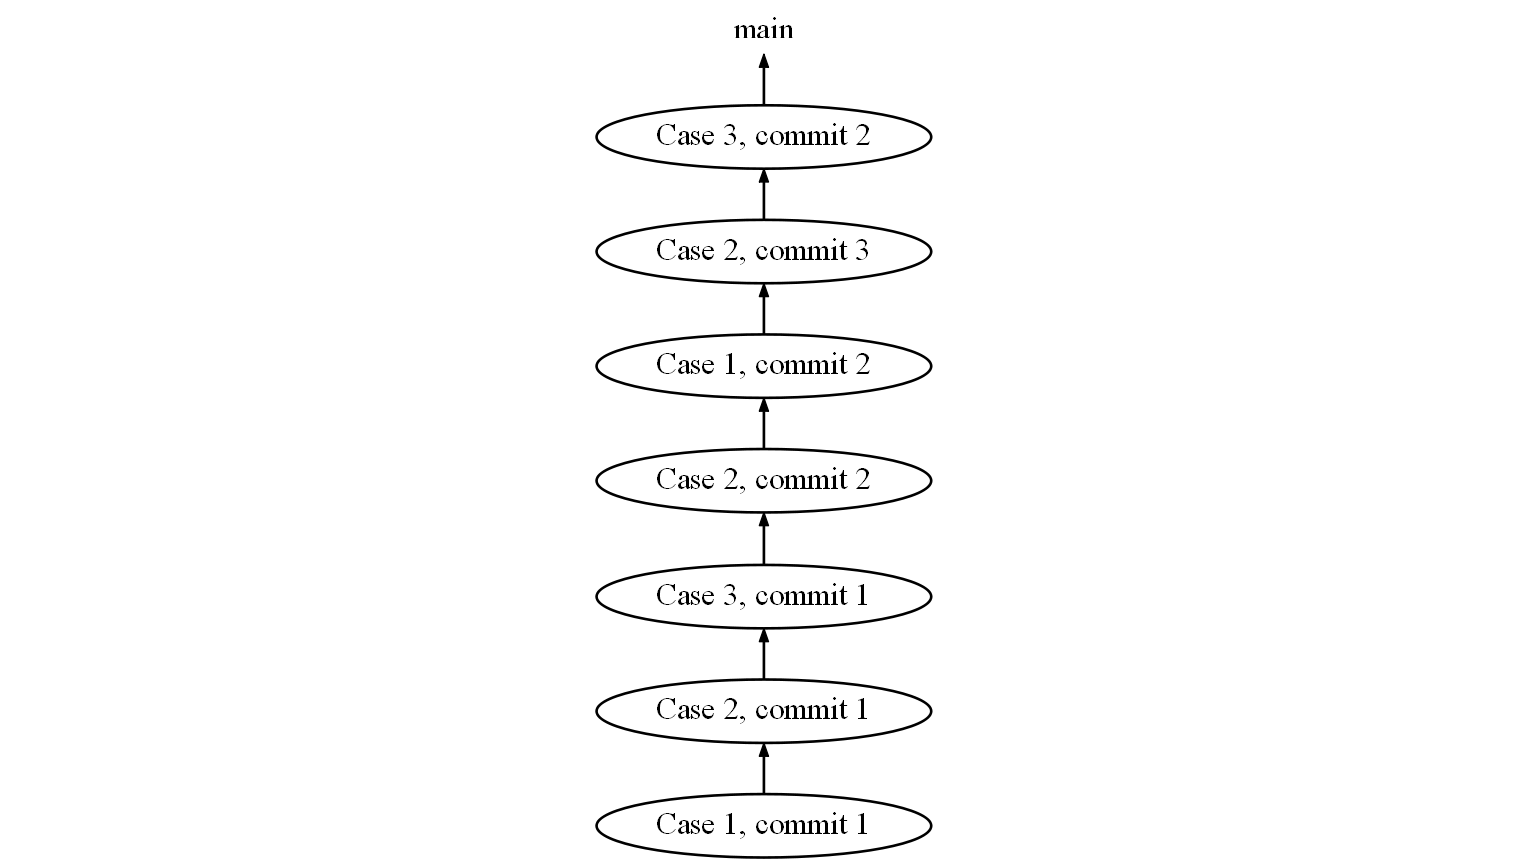
\includegraphics[scale=0.2]{02_2014_only-main.png}
\end{figure}

При ветвлении коммиты группируются по кейсам:
\begin{figure}[h!]
  \centering
  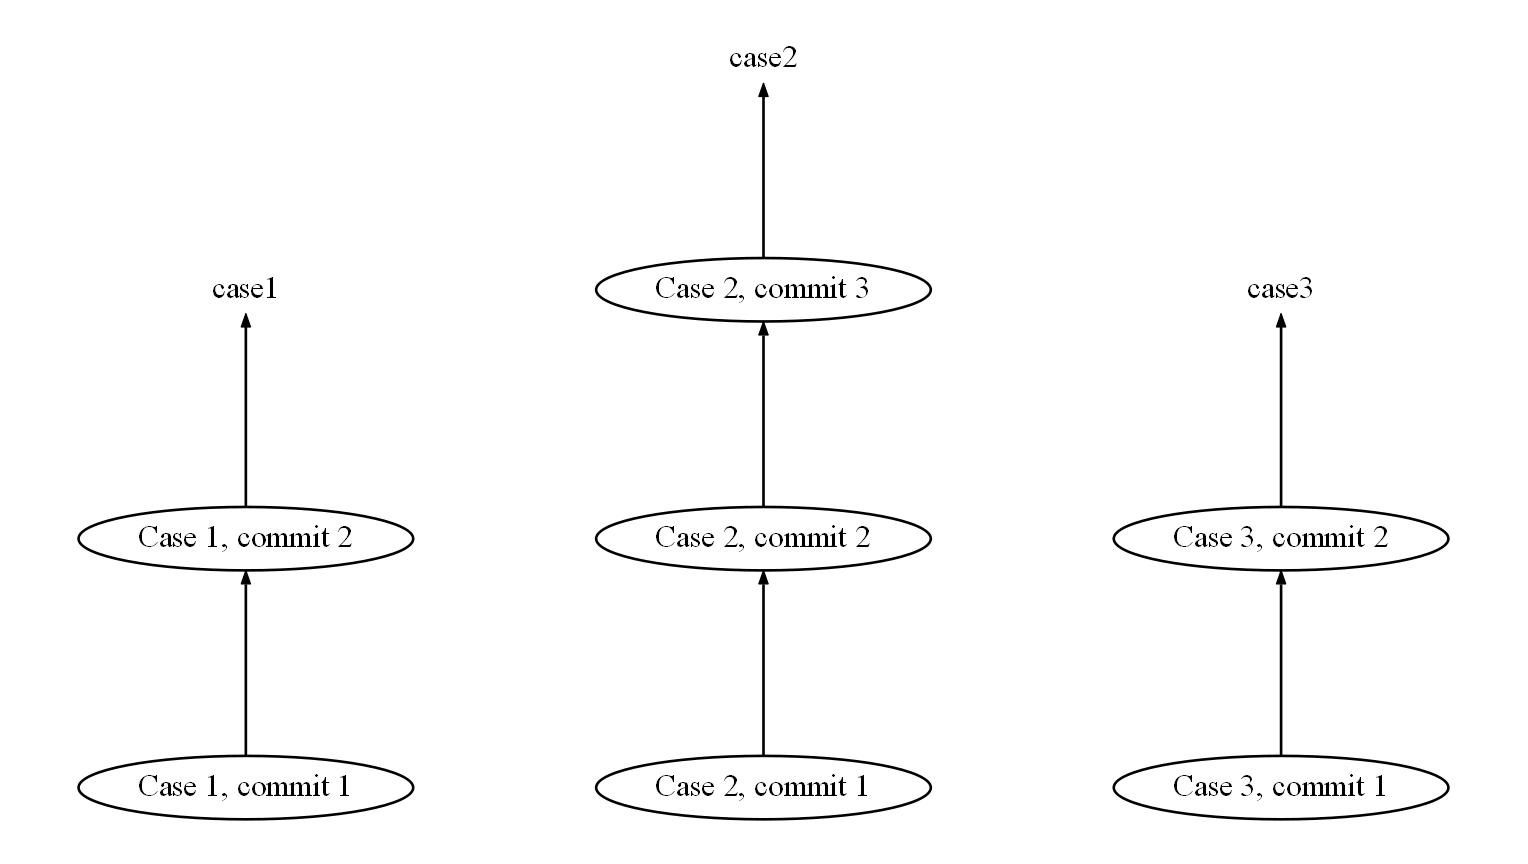
\includegraphics[scale=0.2]{02_2014_branches.png}
\end{figure}

\subsubsection*{Rebasing}

Rebasing может применяться в процессе работы над кейсом, а также для доставки коммитов в mainline.

Rebasing в процессе работы позволяет:

\begin{itemize}
  \item Получить ответвление от обновлённого mainline.
  \item Разрешать merge-conflicts небольшими порциями в ходе работы, а не одним большим куском в самом конце.
  \item Тестировать код своего кейса относительно нового mainline без его доставки в этот самый mainline.
\end{itemize}

Rebase вместо Merge как метод доставки кода в mainline позволяет получить:

\begin{itemize}
  \item Линейную историю в VCS. Линия проще и наглядней графа.
  \item Меньше проблем с blame, bisect и revert. Эти команды работают лучше на коммитах с одним родителем, чем с несколькими.
  \item Возможность удалять очень старые ветки (и их коммиты) из репозитория. Это повышает быстродействие репозитория. А если эти ветки всё-таки нужны "--- их можно хранить в архивном репозитории или в бэкапе. Тем, кто считает замедление репозитория при увеличении количества коммитов надуманной проблемой, есть смысл ознакомиться с исследованием Facebook \cite{Hlebnikov1}.
\end{itemize}

При доставке кода в mainline через Merge, mainline состоит в основном из merge-коммитов:
\begin{figure}[h!]
  \centering
  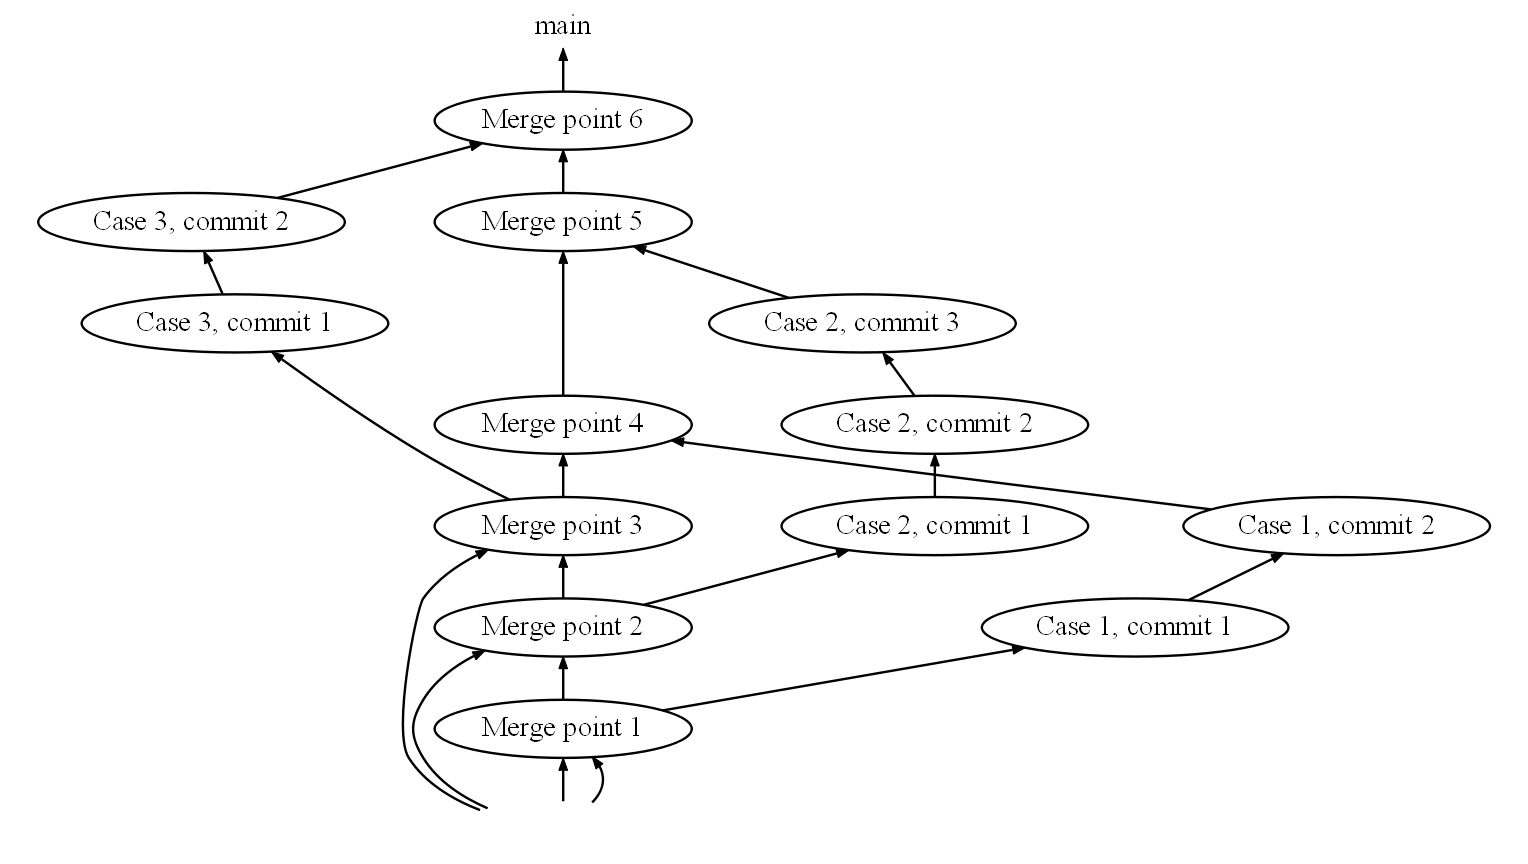
\includegraphics[scale=0.2]{02_2014_main-merged.png}
\end{figure}

Тот же самый граф, но без ярко выраженного вертикального mainline:
\begin{figure}[h!]
  \centering
  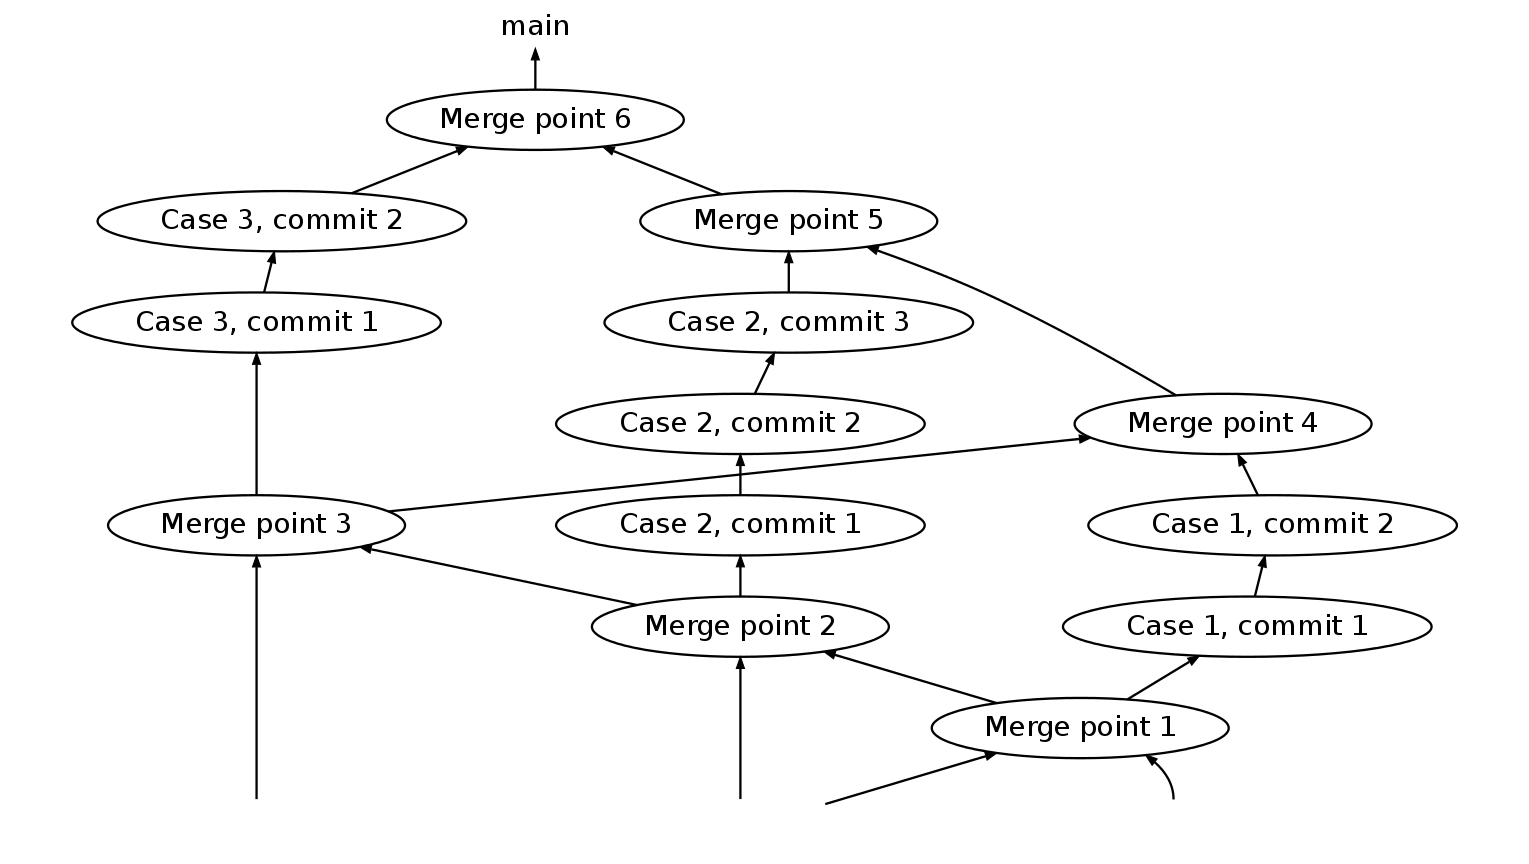
\includegraphics[scale=0.2]{02_2014_main-merged-weak-mainline.png}
\end{figure}

Как видно, в такой истории довольно трудно разобраться, особенно по прошествии долгого времени, или если разбирающийся "--- новый человек на проекте. В этом графе даже mainline трудно найти.

А вот история, которая получается при Rebase:
\begin{figure}[h!]
  \centering
  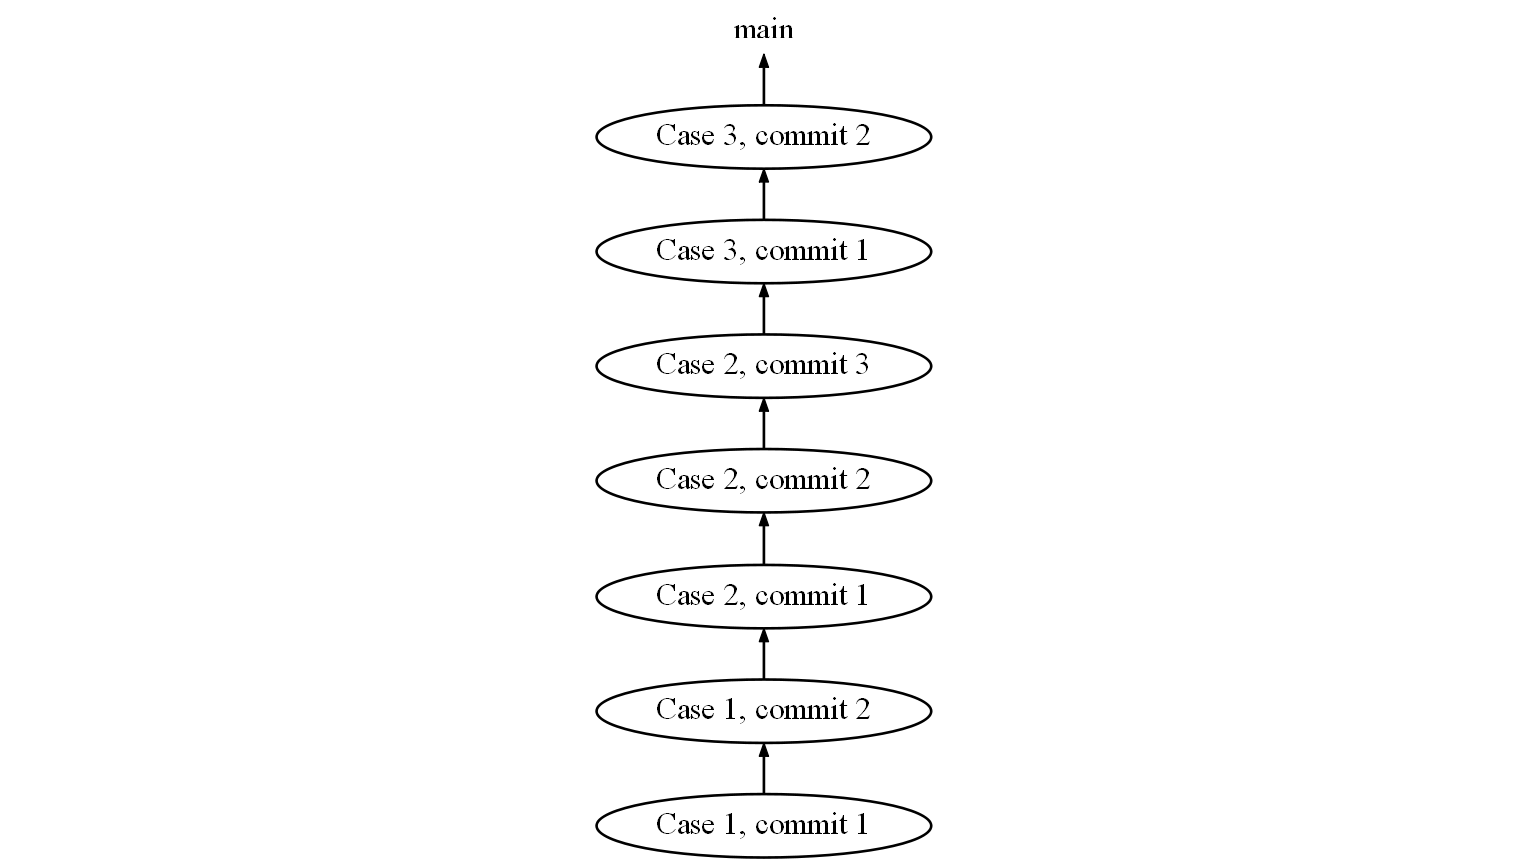
\includegraphics[scale=0.2]{02_2014_main-ordered.png}
\end{figure}

Как видно, история линейна, что сильно улучшает её читаемость. Но можно сделать ещё лучше "--- уменьшить количество коммитов. И в этом поможет squashing.

\subsubsection*{Squashing}

Squashing "--- это слияние нескольких коммитов в один. Squashing позволяет получить:

\begin{itemize}
  \item Компактную историю. Это тем важнее, чем дольше идёт разработка и чем больше коммитов собралось в репозитории.
  \item Меньше мусора в истории.
  \item Более лёгкий откат изменений.
\end{itemize}

Если после работы над кейсом ветка содержит много мусора в истории\ldots{}
\begin{figure}[h!]
  \centering
  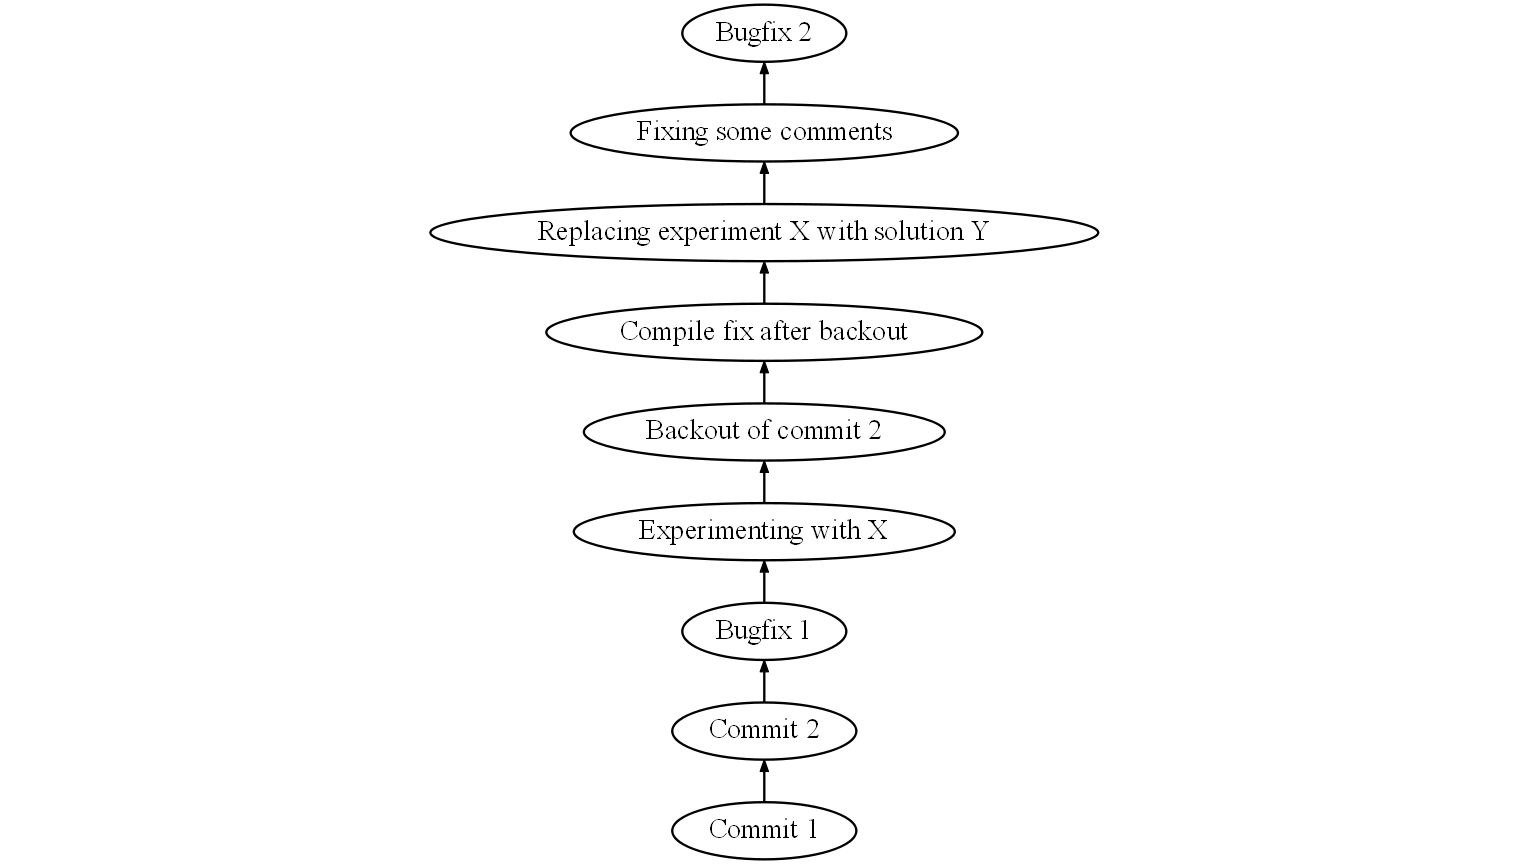
\includegraphics[scale=0.2]{02_2014_history-with-garbage.png}
\end{figure}

\ldots{}squashing позволит избавиться от этого мусора, слив все комиты в один:
\begin{figure}[h!]
  \centering
  
\includegraphics[scale=0.3]{02_2014_history-without-garbage.png}
\end{figure}

\subsection*{Конкретные команды, шаг за шагом}

Приведем примеры команд для Git и Mercurial в виде таблицы:

\begin{table}
  \centering
  \begin{tabular}{P{2.5cm}|P{3.5cm}|P{3.5cm}}
    \hline
                                  ~  & \textbf{Git}                   & \textbf{Mercurial}          \\ \hline
    Ответвление от mainline          & git checkout -{}-b case4       & hg book case4              \\
    Работа над кейсом                & git commit -m "Commit 1" \newline
                                       git commit -m "Commit 2" \ldots{}
                                                                    & hg commit -m "Commit 1" \newline
                                                                      hg commit -m "Commit 2" \ldots{} \\
    Rebase и squash              & git checkout -{}-b \emph{case4-2} \newline
                                   git rebase -{}-interactive main
                                                     & (нужны расширения rebase и histedit) \newline
                                                       hg rebase -{}-keep -{}-dest main \newline
                                                       hg histedit main \newline
                                                       hg book \emph{case4-2}      \\
    \hline
  \end{tabular}
\end{table}
Отдельно коснёмся «табу на rebase после push». Существует довольно распространённый миф, что если ветка запушена (push) на сервер "--- все возможности ребэйса (rebase) для неё потеряны, потому что если ветку проребэйсить и запушить на сервер опять (что возможно только с ключом --force), то это создаст несоответствие между репозиторием на сервере и репозиториями других разработчиков. В результате эти разработчики при попытке подтянуть эту ветку с сервера получат сломанную ветку.

На самом деле rebase возможен, если выполнять его правильно. На примере команд, приведённых в таблице, видно, что при ребэйсинге создаётся новая ветка, \textbf{case4-2}. Это принципиальный момент. Первоначальная ветка, \textbf{case4}, так и остаётся на своём месте, и получается аналог copy-on-write. Таким образом консистентность репозитория не нарушается, и ветка case4 не ломается "--- она просто устаревает. Теперь про неё можно забыть, а дальнейшую разработку, если она ещё продолжается, вести на ветке case4-2.

Также следует обратить внимание на ключ --interactive для Git и команду histedit для Mercurial. В результате их использования Git или Mercurial вызывают текстовый редактор, в котором разработчик может редактировать историю своей ветки: помечать коммиты для правки комментария, сливать несколько коммитов вместе, менять коммиты местами, удалять ненужные коммиты.

В сущности, многие коммиты "--- просто мусор в истории VCS: неудавшиеся эксперименты, багфиксы, фиксы компиляции, чистка неиспользуемых переменных, исправления опечаток в комментариях. Подобный материал в истории VCS не представляет ровным счётом никакого интереса. Как правило, от разработчика требуется имплементация фичи X или исправление бага Y, и желательно одним куском (то есть, как правило (хоть и не всегда), одним коммитом). А детали того, через что разработчик прошёл в процессе разработки, никого не интересуют. По этой причине мелкие правящие коммиты всегда имеет смысл объединить с «главными» коммитами, которые они дополняют. Это же относится и к фиксам в результате code review.

Делать слишком много «главных» коммитов для одного кейса тоже не имеет смысла. Наоборот, для большинства кейсов перед доставкой кода в mainline лучше слить все коммиты в один и использовать название кейса как комментарий этого единственного коммита. Если имел место рефакторинг без изменения функциональности "--- его имеет смысл выделить в отдельный коммит. Если имели место фиксы багов mainline'a, которые проявились при работе над данным кейсом "--- их тоже имеет смысл выделить в отдельные коммиты, и поместить эти коммиты перед основной разработкой. Других коммитов не нужно. Это и есть squashing "--- слияние нескольких коммитов в один.

Кроме чистки мусора в истории squashing также помогает убрать коммиты, которые не компилируются, путём слияния с фиксом компиляции. Это важно, если  используется bisect, а также в случае отката изменений.

Если вам захочется оставить в истории VCS свои чаяния и веяния по поводу данного кейса из ностальгических соображений "--- есть возможность сохранить их только для себя на той старой ветке case4, которая была любезно сохранена при copy-on-write-rebase. Не перетаскивая свой мусор в mainline, разработчик заодно не создает аналогичного искушения для товарищей по команде.

\subsection*{Доставка кода в mainline}

Итак, работа над кейсом завершена, код кейса оттестирован с новейшим mainline. После финальных rebase и squash на ветке должна находиться краткая и красивая история кейса, а сама ветка основана на верхушке mainline. Это и есть подходящий момент для доставки кода кейса в mainline. Для этого надо всего лишь переместить указатель mainline вперёд по ветке case4-2 "--- сделать fast-forward. Это можно сделать несколькими способами; автор предпочитает такие:

\begin{table}
  \centering
  \begin{tabular}{P{3.5cm}|P{6cm}} \hline
    \textbf{Git}                       & \textbf{Mercurial}            \\ \hline
     git push . case4-2:main      & (hg update case4-2) \linebreak
                               hg book main \linebreak  \# «book» does fast-forward \linebreak
                               \# in this case                                               \\ \hline
  \end{tabular}
\end{table}
Важно обратить внимание на точку после git push. Она означает «текущий репозиторий». Однако можно пушить и сразу в origin:

git push origin case4-2:main

При этом не следует опасаться поломки origin/main, т.к. если предлагаемый push не fast-forward, Git не позволит выполнить push без ключа -{}-force.

\subsection*{Выводы}

В результате использования предложенного подхода мы получаем:

\begin{itemize}
  \item Удобство разработки на отдельных ветвях.
  \item Возможность всегда работать и тестировать свои изменения относительно новейшего mainline.
  \item Линейную историю.
  \item Группировку коммитов по кейсам.
  \item Безупречную и компактную историю без мусора.
\end{itemize}

\begin{figure}[h!]
  \centering
  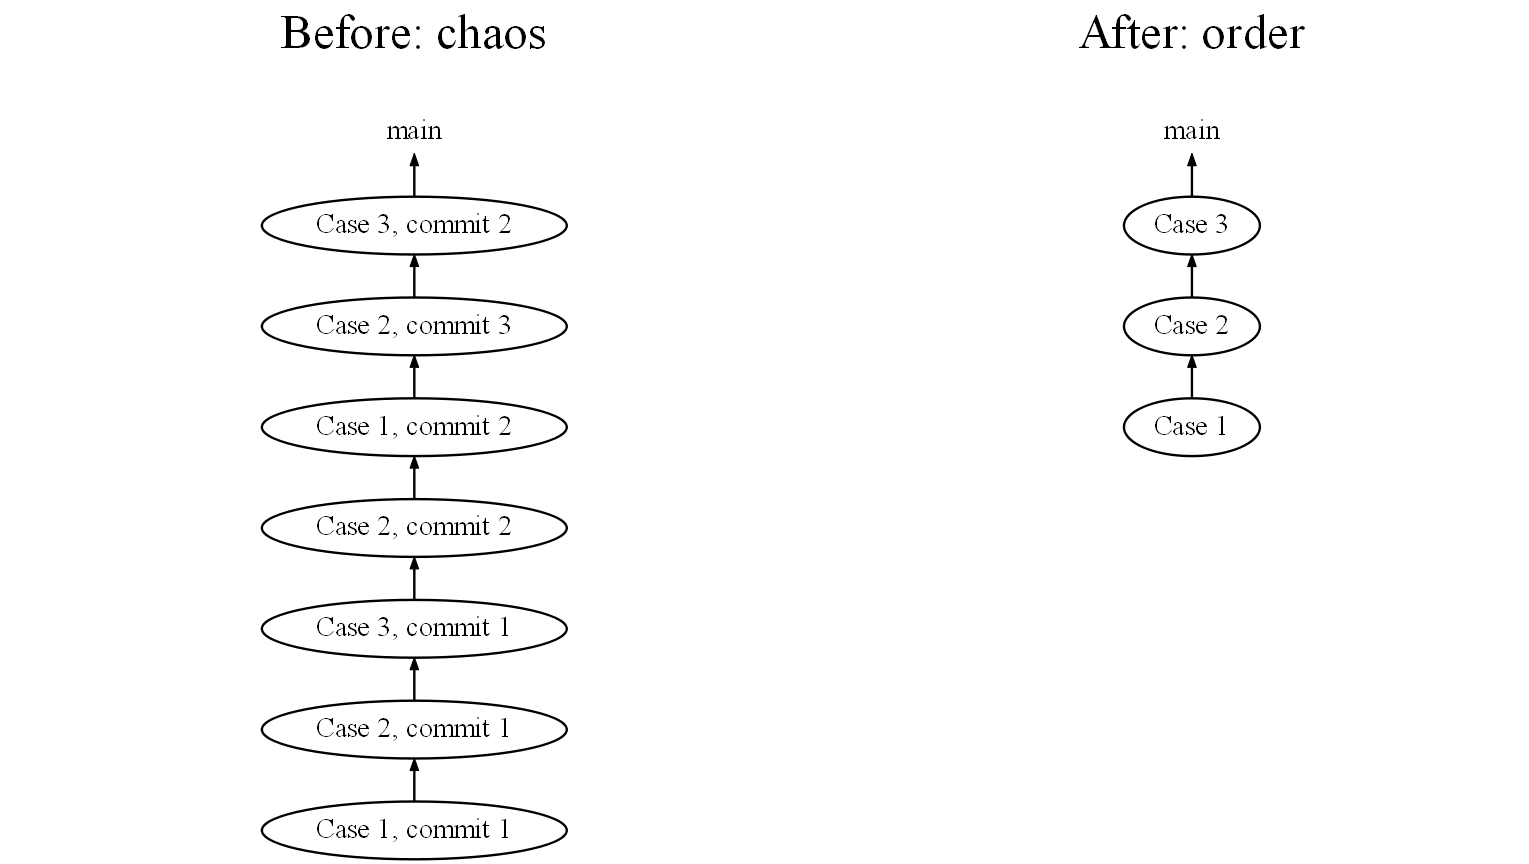
\includegraphics[scale=0.2]{02_2014_before-vs-after.png}
\end{figure}

\begin{thebibliography}{9}
\bibitem{Hlebnikov1} \url{http://thread.gmane.org/gmane.comp.version-control.git/189776}
\end{thebibliography}
\end{document}

\documentclass[10pt, a5paper]{article}
\usepackage{pdfpages}
\usepackage{parallel}
\usepackage[T2A]{fontenc}
\usepackage{ucs}
\usepackage[utf8x]{inputenc}
\usepackage[polish,english,russian]{babel}
\usepackage{hyperref}
\usepackage{rotating}
\usepackage[inner=2cm,top=1.8cm,outer=2cm,bottom=2.3cm,nohead]{geometry}
\usepackage{listings}
\usepackage{graphicx}
\usepackage{wrapfig}
\usepackage{longtable}
\usepackage{indentfirst}
\usepackage{array}
\newcolumntype{P}[1]{>{\raggedright\arraybackslash}p{#1}}
\frenchspacing
\usepackage{fixltx2e} %text sub- and superscripts
\usepackage{icomma} % коскі ў матэматычным рэжыме
\PreloadUnicodePage{4}

\newcommand{\longpage}{\enlargethispage{\baselineskip}}
\newcommand{\shortpage}{\enlargethispage{-\baselineskip}}

\def\switchlang#1{\expandafter\csname switchlang#1\endcsname}
\def\switchlangbe{
\let\saverefname=\refname%
\def\refname{Літаратура}%
\def\figurename{Іл.}%
}
\def\switchlangen{
\let\saverefname=\refname%
\def\refname{References}%
\def\figurename{Fig.}%
}
\def\switchlangru{
\let\saverefname=\refname%
\let\savefigurename=\figurename%
\def\refname{Литература}%
\def\figurename{Рис.}%
}

\hyphenation{admi-ni-stra-tive}
\hyphenation{ex-pe-ri-ence}
\hyphenation{fle-xi-bi-li-ty}
\hyphenation{Py-thon}
\hyphenation{ma-the-ma-ti-cal}
\hyphenation{re-ported}
\hyphenation{imp-le-menta-tions}
\hyphenation{pro-vides}
\hyphenation{en-gi-neering}
\hyphenation{com-pa-ti-bi-li-ty}
\hyphenation{im-pos-sible}
\hyphenation{desk-top}
\hyphenation{elec-tro-nic}
\hyphenation{com-pa-ny}
\hyphenation{de-ve-lop-ment}
\hyphenation{de-ve-loping}
\hyphenation{de-ve-lop}
\hyphenation{da-ta-ba-se}
\hyphenation{plat-forms}
\hyphenation{or-ga-ni-za-tion}
\hyphenation{pro-gramming}
\hyphenation{in-stru-ments}
\hyphenation{Li-nux}
\hyphenation{sour-ce}
\hyphenation{en-vi-ron-ment}
\hyphenation{Te-le-pathy}
\hyphenation{Li-nux-ov-ka}
\hyphenation{Open-BSD}
\hyphenation{Free-BSD}
\hyphenation{men-ti-on-ed}
\hyphenation{app-li-ca-tion}

\def\progref!#1!{\texttt{#1}}
\renewcommand{\arraystretch}{2} %Іначай формулы ў матрыцы зліпаюцца з лініямі
\usepackage{array}

\def\interview #1 (#2), #3, #4, #5\par{

\section[#1, #3, #4]{#1 -- #3, #4}
\def\qname{LVEE}
\def\aname{#1}
\def\q ##1\par{{\noindent \bf \qname: ##1 }\par}
\def\a{{\noindent \bf \aname: } \def\qname{L}\def\aname{#2}}
}

\def\interview* #1 (#2), #3, #4, #5\par{

\section*{#1\\{\small\rm #3, #4. #5}}

\def\qname{LVEE}
\def\aname{#1}
\def\q ##1\par{{\noindent \bf \qname: ##1 }\par}
\def\a{{\noindent \bf \aname: } \def\qname{L}\def\aname{#2}}
}

\begin{document}
\title{Коммерциализаия СПО под GPL лицензией}
\author{Александр Рябиков, Сергей Середа "--- Москва, РФ\footnote{\url{rsashka@mail.ru}, \url{http://lvee.org/en/abstracts/121}}}
\maketitle
\begin{abstract}
In accordance to main goals of ADempiere Foundation our task was to find a way to get return on investments in Free Software modification/enhancement for a SMB developer company without dual licensing and without accompanying the product with proprietary add"=ons/plugins or additional services or merchandise. Also there were a need to provide a mechanism of costs' sharing between several interested SMB companies.

After initial economic analysis we've concluded that the only way to get return on investments in free software development is to create a time lag between the moment of software product provision to a user and the moment of rights provision for this software according to GPL. Otherwise, demand and supply law just will not work with free software.

Also we have studied the legislation and FSF Comprehensive FAQ about the GNU Licenses. As a result, there were constructed two schemes that could create such time lag without GPL violation. 

First is based mostly on GNU FAQ, second is based on the provisions of contract law.
\end{abstract}
%\begin{center}\textbf{Фонд поддержки и развития делового свободного программного обеспечения ``Адемпиере''}\end{center}

%\begin{flushright}Авторы: 
%Александр Рябиков, 
%Сергей Середа, к.э.н.,\end{flushright}

\subsection*{СПО под GPL лицензией}

Как известно, “свободные” лицензии дают конечным пользователям полную свободу, в том числе и свободу распространять конечный программный продукт наравне с разработчиком. А это означает, что каждый раз, когда разработчик продаёт копию ПО под “свободной” лицензией, он создает себе конкурента. Принято считать, что невозможно зарабатывать деньги непосредственно на доработке и распространении свободного программного обеспечения, распространяемого на условиях GPL или совместимых с нею лицензий. Описываемые в литературе и применяемые на практике бизнес"=модели практически безусловно предполагают бесплатное (или за символическую плату) распространение таких программ. В противоположность этому, наличие “традиционной” (на жаргоне называемой “проприетарной”) лицензии позволяет зарабатывать непосредственно на распространении программного обеспечения.

Обладателю исключительных прав на программу ещё доступна модель двойного лицензирования, подразумевающая “несвободную” коммерческую лицензию на ПО для бизнес"=заказчиков и GPL"=совместимую лицензию  для представителей сообщества. Для всех же вторичных проектов (так называемых “форков”) подобная возможность исключена. Любые доработки кода для ПО, выпущенного под GPL, могут быть выпущены только под этой же или совместимой “вирусной” лицензией, а замена GPL на несовместимую лицензию допускается только с согласия всех обладателей исключительных прав на программу.

С учетом этого, считается, что зарабатывать на Free Software, не являясь обладателем прав на оригинальный продукт, можно либо оказывая сервисные услуги (сопровождение, документирование, обучение и т.п.), либо компонуя его с собственными разработками с закрытым исходным кодом, способом, который допускается используемой свободной лицензией.

Описываемый ниже способ коммерциализации доработок свободного ПО позволит в определенной мере изменить сложившуюся ситуацию. Предлагаемая бизнес"=модель предназначена, в основном для b2b"=разработчиков, развивающих уже существующие свободные программные продукты, но не владеющих исключительным правом на сам продукт (т.е. наиболее часто встречающаяся ситуация).

Суть бизнес"=модели сводится к созданию условий, аналогичных “традиционному” модели распространения программного обеспечения, т.е. к “продаже” доработанного продукта сразу нескольким покупателям, что даст возможность окупить понесенные затраты на доработку СПО за счет их многократной продажи. Такой эффект достигается за счет создания временного лага между началом продаж доработанного программного продукта и моментом его размещения в свободном доступе для бесплатной загрузки, что позволяет разработчику стать, на какое"=то время, единственным продавцом, у кого эти доработки можно будет приобрести.

Особенность предлагаемой модели заключается в том, что при этом не происходит ни изменения, ни нарушения условий “вирусного” лицензионного соглашения "--- эффективное ограничение распространения продукта определяется договором между хозяйствующими субъектами и вытекает из процесса выполнения заказных программных разработок.

\subsection*{1. Решение, «подсказанное» Free Software \linebreak Foundation (FSF)}

Временной лаг создаётся за счёт превращения пользователя в (со)разработчика, подписания с ним соглашения о нераспространении экземпляров продукта и предоставления ему программного обеспечения для тестирования на продуктивных данных.

\subsubsection*{Часто забываемые факты о GPL}

\begin{itemize}
  \item GPL допускает платное распространение программ \cite{ryabikov1}.
  \item GPL не требует от разработчика делать исходные коды своих разработок доступными широкой публике \cite{ryabikov2}.
  \item Разработчик не вправе запрещать Заказчику дальнейшее распространение ПО \cite{ryabikov3, ryabikov4}.
  \item GPL позволяет Заказчику запретить разработчику распространять результаты заказной разработки  \cite{ryabikov5}.
\end{itemize}

\subsection*{Сценарий по «подсказке» FSF}

Исходная ситуация: Разработчиком доработан GPL"=продукт, \linebreak есть компания"=пользователь, желающая внедрить доработанный \linebreak продукт, но не готовая оплатить полную стоимость доработки, Разработчику необходимо обеспечить возврат инвестиций в доработку, но есть риск, что компания"=пользователь опубликует доработки, как только получит к ним доступ.

\subsubsection*{Предлагаемая схема взаимодействия к компанией"=пользователем:}

\begin{itemize}
  \item Разработчик продает компании"=пользователю исходный продукт без своих доработок.
  \item Разработчик нанимает компанию"=пользователя для выполнения работ, связанных с новым кодом, в частности, для тестирования.
  \item В соответствии с комментариями FSF \cite{ryabikov5} существует законная возможность ограничить распространение тестируемого кода на время действия соответствующего договора.
  \item Время действия этого договора и будет определять временной лаг между началом распространения доработок GPL продукта и моментом его появления в свободном доступе.
  \item Разработчик может одновременно работать по такой схеме сразу с несколькими заинтересованными компаниями.
\end{itemize}

\subsection*{2. Решение на основе договорного права}

Временной лаг создаётся за счёт того, что права на созданный по заказу код и возможность его дальнейшего распространения возникают только после полного исполнения обязательств сторонами договора на доработку ПО.

\subsubsection*{Сценарий на основе договорного права}

Исходная ситуация: Разработчиком доработан GPL"=продукт \linebreak  (разработчик готов его доработать), есть компания"=пользователь, желающая внедрить доработанный продукт, но не готовая оплатить полную стоимость доработки, Разработчику необходимо обеспечить возврат инвестиций в доработку, но есть риск, что компания"=пользователь опубликует доработки, как только получит к ним доступ.

\subsubsection*{Предлагаемая схема взаимодействия к компанией"=пользователем:}

\begin{itemize}
  \item Разработчик заключает с компанией"=пользователем договор на доработку исходного GPL продукта.
  \item В соответствии с действующим законодательством РФ (Статья 712. Право подрядчика на удержание, Статья 1296. Программы для ЭВМ и базы данных, созданные по заказу), в этом случае существует законная возможность ограничить распространение тестируемого кода на время действия соответствующего договора.
  \item Время действия этого договора и будет определять временной лаг между началом распространения доработок продукта под GPL лицензией и моментом его появления в свободном доступе.
  \item Разработчик может одновременно работать по такой схеме сразу с несколькими заинтересованными компаниями.
\end{itemize}

Описанная конструкция не является каким"=то искусственным построением. Наоборот, она является описанием вполне реального процесса заказной разработки корпоративного ПО, который завершается только после проведения опытной или опытно"=промышленной эксплуатации разработок (с их полным сопровождением все это время) и передачи их в промышленную эксплуатацию.

По мнению авторов, регулируя длительность временного лага между началом продаж доработанного программного продукта и моментом его размещения в свободном доступе для бесплатной загрузки, в зависимости от типа, сложности, популярности и иных характеристик дорабатываемого программного продукта, можно обеспечить возврат инвестиций в его развитие, достаточный для поддержания коммерческого предприятия. При этом, за счет заключения подобных договоров с несколькими (в идеале "--- со многими) пользователями"=заказчиками будет также обеспечено и разделение затрат между ними (в отличие от схемы bounty source, в рамках которой доработка целиком оплачивается одним заказчиком).

Конечно, наложение любых ограничений на распространение СПО может быть воспринято “в штыки” сообществом и, возможно, потребуются определенные усилия, что бы сторонники двух диаметрально противоположных точек зрения на способы распространения ПО смогли оценить положительные и отрицательные стороны от такого “нововведения”. Тем не менее, описанная бизнес"=модель полностью основана на законе и не нарушает ни одного положения о защите интеллектуальной собственности. Более того, она, по сути, является просто специализированной модификацией широко применяемой в корпоративном секторе стандартной модели заказной разработки ПО.

Мы обсудили с Ричардом Столлманом эти способы и он сделал важные замечания к описываемым моделям. Второй способ на основе контрактного права соответствует GPLv2, но нарушает GPLv3, где в явном виде прописано, что лицензия имеет приоритет над контрактными обязательствами. С этим мнением не согласны наши юристы, но кто из них прав может решить только судебная практика.
Насчет первого способа, Ричард конечно не в восторге, но нарушение GPL будет в том случае, если работа пользователя будет фиктивной. Другими словами, пользователь должен по настоящему работать в соответствии с контрактными обязательствами и эта работа должна реально оплачиваться.

Конечно, используя описанные выше принципы, первое время код будет отсутствовать в свободном доступе, но через какое то время он все равно станет доступен для всех. И в результате, и инвесторы вернут вложенные средства и сообщество получит ощутимый вклад в развитие СПО.

Данная методика коммерциализации СПО с лицензией GPL была представлена на Russian Open Source Summit 2014. Статья по материалам доклада доступна на сайте PCWEEK \cite{ryabikov6}.

\begin{thebibliography}{9}
\bibitem{ryabikov1} \url{http://www.gnu.org/licenses/gpl-faq.en.html#DoesTheGPLAllowMoney}
\bibitem{ryabikov2} \url{http://www.gnu.org/licenses/gpl-faq.en.html#DoesTheGPLRequireAvailabilityToPublic}
\bibitem{ryabikov3} \url{http://www.gnu.org/licenses/gpl-faq.en.html#DoesTheGPLAllowNDA}
\bibitem{ryabikov4} \url{http://www.gnu.org/licenses/gpl-faq.en.html#DoesTheGPLAllowModNDA}
\bibitem{ryabikov5} \url{http://www.gnu.org/licenses/gpl-faq.en.html#DevelopChangesUnderNDA}
\bibitem{ryabikov6} \url{http://www.pcweek.ru/foss/article/detail.php?ID=164583}
\end{thebibliography}
\end{document}

%\input{01_2014_LastName}
%%%\chapter{LVEE Winter 2014}
%\input{101_2014_w_LastName}
%\documentclass[10pt, a5paper]{article}
\usepackage{pdfpages}
\usepackage{parallel}
\usepackage[T2A]{fontenc}
\usepackage{ucs}
\usepackage[utf8x]{inputenc}
\usepackage[polish,english,russian]{babel}
\usepackage{hyperref}
\usepackage{rotating}
\usepackage[inner=2cm,top=1.8cm,outer=2cm,bottom=2.3cm,nohead]{geometry}
\usepackage{listings}
\usepackage{graphicx}
\usepackage{wrapfig}
\usepackage{longtable}
\usepackage{indentfirst}
\usepackage{array}
\newcolumntype{P}[1]{>{\raggedright\arraybackslash}p{#1}}
\frenchspacing
\usepackage{fixltx2e} %text sub- and superscripts
\usepackage{icomma} % коскі ў матэматычным рэжыме
\PreloadUnicodePage{4}

\newcommand{\longpage}{\enlargethispage{\baselineskip}}
\newcommand{\shortpage}{\enlargethispage{-\baselineskip}}

\def\switchlang#1{\expandafter\csname switchlang#1\endcsname}
\def\switchlangbe{
\let\saverefname=\refname%
\def\refname{Літаратура}%
\def\figurename{Іл.}%
}
\def\switchlangen{
\let\saverefname=\refname%
\def\refname{References}%
\def\figurename{Fig.}%
}
\def\switchlangru{
\let\saverefname=\refname%
\let\savefigurename=\figurename%
\def\refname{Литература}%
\def\figurename{Рис.}%
}

\hyphenation{admi-ni-stra-tive}
\hyphenation{ex-pe-ri-ence}
\hyphenation{fle-xi-bi-li-ty}
\hyphenation{Py-thon}
\hyphenation{ma-the-ma-ti-cal}
\hyphenation{re-ported}
\hyphenation{imp-le-menta-tions}
\hyphenation{pro-vides}
\hyphenation{en-gi-neering}
\hyphenation{com-pa-ti-bi-li-ty}
\hyphenation{im-pos-sible}
\hyphenation{desk-top}
\hyphenation{elec-tro-nic}
\hyphenation{com-pa-ny}
\hyphenation{de-ve-lop-ment}
\hyphenation{de-ve-loping}
\hyphenation{de-ve-lop}
\hyphenation{da-ta-ba-se}
\hyphenation{plat-forms}
\hyphenation{or-ga-ni-za-tion}
\hyphenation{pro-gramming}
\hyphenation{in-stru-ments}
\hyphenation{Li-nux}
\hyphenation{sour-ce}
\hyphenation{en-vi-ron-ment}
\hyphenation{Te-le-pathy}
\hyphenation{Li-nux-ov-ka}
\hyphenation{Open-BSD}
\hyphenation{Free-BSD}
\hyphenation{men-ti-on-ed}
\hyphenation{app-li-ca-tion}

\def\progref!#1!{\texttt{#1}}
\renewcommand{\arraystretch}{2} %Іначай формулы ў матрыцы зліпаюцца з лініямі
\usepackage{array}

\def\interview #1 (#2), #3, #4, #5\par{

\section[#1, #3, #4]{#1 -- #3, #4}
\def\qname{LVEE}
\def\aname{#1}
\def\q ##1\par{{\noindent \bf \qname: ##1 }\par}
\def\a{{\noindent \bf \aname: } \def\qname{L}\def\aname{#2}}
}

\def\interview* #1 (#2), #3, #4, #5\par{

\section*{#1\\{\small\rm #3, #4. #5}}

\def\qname{LVEE}
\def\aname{#1}
\def\q ##1\par{{\noindent \bf \qname: ##1 }\par}
\def\a{{\noindent \bf \aname: } \def\qname{L}\def\aname{#2}}
}

\begin{document}
\title{Голос спонсора: SaM Solutions}
%\author{}
\date{}
\maketitle

Компания SaM Solutions выступает в роли системо-образующего спонсора конференции Linux Vacation Eastern Europe с момента рождения LVEE в 2005 году и на протяжении всех лет её проведения. 

Сложившаяся корпоративная практика не случайна. Продукты и решения, задействующие Linux и другие Free/Open Source Software проекты, составляют заметную часть пакета разработок SaM Solutions. Кадровая политика компании направлена на поощрение профессионального развития своих сотрудников, организацию их эффективного отдыха и привлечение хорошо мотивированных кандидатов к работе на компанию. Формат конференции LVEE успешно позволяет решать все три задачи. 

Одним из подразделений компании является отдел Linux и \linebreak Embbeded. Специалисты компании на протяжении десятилетий работают с СПО. Компанией реализован ряд проектов по адаптации ОС GNU/Linux для работы в различных устройствах, построенных на таких платформах как ARM, PowerPC, x86, MIPS. В последние годы "--- на ведущие позиции выходит разработка управляющего ПО для серверов Enterprise-класса, от низкоуровнего BMC Firmware на основе Linux до высокоуровневых систем контроля виртуализации и графических интерфейсов управления, от прошивок устройств хранения данных до BSP интегрированных плат для разработчика. Надёжность, качество и широкая функциональность множества свободных проектов позволяет строить нам системы любого уровня и сложности, опираясь на высококачественные готовые компоненты.

В рамках направления Linux и Embedded успешно выполнены проекты для таких знаковых заказчиков, как  Novell/SUSE, Fujitsu Technology Solutions  и осуществляется партнёрство с компаниями IBM и Oracle/Sun в области Open Source решений.

Мы разрабатываем, модифицируем и адаптируем различное свободное программное обеспечение для наших заказчиков, но не забываем и о своих нуждах "--- наши сотрудники используют в своей работе существующие програмные продукты и вносят вклад в их развитие. Часть внутренней инфраструктуры, а именно интранет-сеть компании, тестовые стенды отдела контроля качества, рабочие места сотрудников профильных подразделений "--- также работает под управлением СПО (серверные и десктопные платформы GNU/Linux и FreeBSD). 

В минувшем году, в рамках реорганизации, был разработан долгосрочный план развития направления Linux и Embedded в SaM Solutions. В нём впервые были кодифицированы уже имеющиеся внутренние неофициальные практики по взаимодействию с commu"=nity-based проектами. В частности разработаны меры и правила по
\begin{itemize}
  \item возврата изменений в родительские проекты (upstreaming);
  \item вхождения в состав постоянных разработчиков активно используемых нами FOSS-компонентов;
  \item публикации сообщений об ошибках (bug reporting);
  \item участия и помощи в организации community events;
  \item стимуляции докладов и участия в технических конференциях.
\end{itemize}
И план немедленно начал претворяться в жизнь.

Силами отдела организовано внутреннее обучение сотрудников на регулярной
основе. Был прочтен и опубликован курс по TDD. По согласованию с автором
опубликован курс Debian/Ubuntu Packaging (видео, презентация и исходные
тексты презентации в \LaTeX).  Были организованы и проведены курсы по
обучению QA специалистов для направления Embeded Linux. Проведено
практическое занятие по основам виртуализации и эмуляции, организована
лекция по вопросу профилирования и оптимизации Ruby-кода, лекция о
High-availability кластерах и направлении развития технологии. Кроме того,
проводился семинар по Video4Linux2. Для создания и обучения кадрового
резерва на ближайшее будущее запланированы постоянно действующие внутренние
проекты в области Embedded Linux, результаты которых также запланированы к
публикации.

Визиты представительных делегаций на Embedded World 2012 и Linux Con Europe/Embedded LinuxCon Europe 2011 обогатили нас новыми идеями, куда можно
двигаться дальше и что сейчас актуально. А выступления на Software
Engineering Forum for Students, круглом столе по СПО в рамках TIBO-2012
и LVEE Winter 2012 позволили поделиться опытом с
заинтересованными сторонами.

В апреле состоялась Ганноверская промышленная ярмарка \linebreak (Hannover Messe
2013). Компания SaM Solutions была представлена отдельным стендом, на
котором демонстрировались наработки в области встроенного и системного ПО
на базе OS Linux. Идея «умного» дома вызвала неподдельный интерес у
посетителей стенда.

При поддержке SaM Solutions, с декабря 2011 года возобновились регулярные встречи Minsk Linux Users Groups, под названием <<Линуксовка в SaM Solutions>>. Техническое оснащение линуксовок и открытый формат встреч позволил им практически мгновенно стать заметным дискуссионным клубом по широкому спектру вопросов, прямо или косвенно связанных с СПО. Свободная картография (OpenStreetMap), технологии виртуализации, минский \linebreak hackerspace, Linux Mobile, бойкот Голливудской продукции, systemd, загрузчик u-boot, белорусская локализация GNOME --- это только часть тем, поднятых за последние линуксовки.

Быстрые и положительные изменения, как внутри компании SaM Solutions, так и в экосфере СПО (и Linux в частности) наполняют нас уверенностью, что направление движения выбрано верно.

\begin{figure}[h!]
\centering

\includegraphics[height=11.8cm]{48_spons_sams.pdf}
\end{figure}
\end{document}



%\documentclass[10pt, a5paper]{article}
\usepackage{pdfpages}
\usepackage{parallel}
\usepackage[T2A]{fontenc}
\usepackage{ucs}
\usepackage[utf8x]{inputenc}
\usepackage[polish,english,russian]{babel}
\usepackage{hyperref}
\usepackage{rotating}
\usepackage[inner=2cm,top=1.8cm,outer=2cm,bottom=2.3cm,nohead]{geometry}
\usepackage{listings}
\usepackage{graphicx}
\usepackage{wrapfig}
\usepackage{longtable}
\usepackage{indentfirst}
\usepackage{array}
\newcolumntype{P}[1]{>{\raggedright\arraybackslash}p{#1}}
\frenchspacing
\usepackage{fixltx2e} %text sub- and superscripts
\usepackage{icomma} % коскі ў матэматычным рэжыме
\PreloadUnicodePage{4}

\newcommand{\longpage}{\enlargethispage{\baselineskip}}
\newcommand{\shortpage}{\enlargethispage{-\baselineskip}}

\def\switchlang#1{\expandafter\csname switchlang#1\endcsname}
\def\switchlangbe{
\let\saverefname=\refname%
\def\refname{Літаратура}%
\def\figurename{Іл.}%
}
\def\switchlangen{
\let\saverefname=\refname%
\def\refname{References}%
\def\figurename{Fig.}%
}
\def\switchlangru{
\let\saverefname=\refname%
\let\savefigurename=\figurename%
\def\refname{Литература}%
\def\figurename{Рис.}%
}

\hyphenation{admi-ni-stra-tive}
\hyphenation{ex-pe-ri-ence}
\hyphenation{fle-xi-bi-li-ty}
\hyphenation{Py-thon}
\hyphenation{ma-the-ma-ti-cal}
\hyphenation{re-ported}
\hyphenation{imp-le-menta-tions}
\hyphenation{pro-vides}
\hyphenation{en-gi-neering}
\hyphenation{com-pa-ti-bi-li-ty}
\hyphenation{im-pos-sible}
\hyphenation{desk-top}
\hyphenation{elec-tro-nic}
\hyphenation{com-pa-ny}
\hyphenation{de-ve-lop-ment}
\hyphenation{de-ve-loping}
\hyphenation{de-ve-lop}
\hyphenation{da-ta-ba-se}
\hyphenation{plat-forms}
\hyphenation{or-ga-ni-za-tion}
\hyphenation{pro-gramming}
\hyphenation{in-stru-ments}
\hyphenation{Li-nux}
\hyphenation{sour-ce}
\hyphenation{en-vi-ron-ment}
\hyphenation{Te-le-pathy}
\hyphenation{Li-nux-ov-ka}
\hyphenation{Open-BSD}
\hyphenation{Free-BSD}
\hyphenation{men-ti-on-ed}
\hyphenation{app-li-ca-tion}

\def\progref!#1!{\texttt{#1}}
\renewcommand{\arraystretch}{2} %Іначай формулы ў матрыцы зліпаюцца з лініямі
\usepackage{array}

\def\interview #1 (#2), #3, #4, #5\par{

\section[#1, #3, #4]{#1 -- #3, #4}
\def\qname{LVEE}
\def\aname{#1}
\def\q ##1\par{{\noindent \bf \qname: ##1 }\par}
\def\a{{\noindent \bf \aname: } \def\qname{L}\def\aname{#2}}
}

\def\interview* #1 (#2), #3, #4, #5\par{

\section*{#1\\{\small\rm #3, #4. #5}}

\def\qname{LVEE}
\def\aname{#1}
\def\q ##1\par{{\noindent \bf \qname: ##1 }\par}
\def\a{{\noindent \bf \aname: } \def\qname{L}\def\aname{#2}}
}

\begin{document}
\title{Голос спонсора: EPAM Systems}
%\author{}
\date{}
\maketitle

Компания EPAM Systems не первый год является спонсором международной конференции разработчиков и пользователей свободного программного обеспечения LVEE (Linux Vacation / Eastern Europe). Этот год также не стал исключением. Пожалуй, LVEE является самым значимым событием для русскоязычных разработчиков и тестировщиков Open Source. Каждое лето здесь встречаются начинающие специалисты и «ветераны»"=разработчики из десятка стран для обмена опытом и общения на профессиональные темы. Наши специалисты также активно участвуют в данной конференции: в качестве докладчиков и организаторов/волонтёров. Это уникальная в своём роде конференция, и именно поэтому EPAM Systems очередной раз принимает участие в LVEE в качестве спонсора.


EPAM Systems "--- одна из крупнейших компаний"=поставщиков\linebreak услуг в области разработки программного обеспечения и решений на территории СНГ и Центральной и Восточной Европы. Созданная в 1993 году, сегодня она имеет представительства в 12 странах мира, в штате работают более 9 тыс. сотрудников, из которых более 3 тыс. "--- в Беларуси. Рост компании обеспечивается за счет собственных обучающих программ и передаче опыта от больших специалистов до начинающих разработчиков. Компания EPAM Systems выполняет проекты более чем в 30 странах мира. Основные направления деятельности: разработка, тестирование, сопровождение и поддержка заказного программного обеспечения и бизнес"=приложений, а также ИТ"=консалтинг с учетом отраслевой специфики бизнеса.

Наша компания участвует в проектах с такими крупными, хорошо известными заказчиками как Google, Novell, Infoblox, Parallels, 10Gen и др., так и с небольшими, в том числе и с начинающими свой путь в софтверном бизнесе.


К примеру, для Infoblox была реализована связка между WebUI с BIND и DHCP. Для этого был разработан комплекс решений под управлением Shell и Python скриптов, а также механизм позволяющий вносить правки в BIND и DHCP на языке C. Также был разработан развернутый функционал, автоматизирующий инсталляцию новых устройств и их эксплуатацию, что позволяет значительно упростить управление данными. Встроенный Web"=интерфейс позволяет разворачивать, управлять сервисами DNS, DNSSEC, DHCP, IPAM, устанавливать новые версии ПО, архивировать и восстанавливать из архивов необходимые данные, восстанавливать их после аварии, проводить мониторинг сети и создавать отчеты без необходимости обращения к командной строке.


Еще одним решением, реализованным для компании Infoblox, являлся программный продукт, позволяющий контролировать сетевые изменения, таким образом, облегчая идентификацию трудноуловимых проблем конфигурации и соответствие требованиям. Вместо того чтобы просто регистрировать изменения, система использует внесенную информацию для проверки, анализа и автоматической обработки сетевых изменений. Благодаря инновационной, квалифицированной, глубокой технике логического анализа, программа изолирует проблемы исправности и конфигурации до того, как они могут вызвать более серьезные сбои.


Разработанная для анализа сложных сетей система изучает сеть, собирает ключевую информацию, применяет встроенную технику логического анализа и создает оценку исправности сети и список проблем, требующих принятие мер для улучшения качества работы сети.


Правильное использование свободного ПО в разработках сокращает и расходы на покупку лицензионных программ, и трудозатраты при создании коммерческого ПО. Немалую роль для достижения превосходного результата играет привлечение к разработке опытных специалистов. LVEE способствует появлению таких специалистов, развитию их навыков и расширению кругозора. Хотелось бы пожелать участникам конференции интересных проектов и максимум пользы от участия в LVEE.


\end{document}



%\documentclass[10pt, a5paper]{article}
\usepackage{pdfpages}
\usepackage{parallel}
\usepackage[T2A]{fontenc}
\usepackage{ucs}
\usepackage[utf8x]{inputenc}
\usepackage[polish,english,russian]{babel}
\usepackage{hyperref}
\usepackage{rotating}
\usepackage[inner=2cm,top=1.8cm,outer=2cm,bottom=2.3cm,nohead]{geometry}
\usepackage{listings}
\usepackage{graphicx}
\usepackage{wrapfig}
\usepackage{longtable}
\usepackage{indentfirst}
\usepackage{array}
\newcolumntype{P}[1]{>{\raggedright\arraybackslash}p{#1}}
\frenchspacing
\usepackage{fixltx2e} %text sub- and superscripts
\usepackage{icomma} % коскі ў матэматычным рэжыме
\PreloadUnicodePage{4}

\newcommand{\longpage}{\enlargethispage{\baselineskip}}
\newcommand{\shortpage}{\enlargethispage{-\baselineskip}}

\def\switchlang#1{\expandafter\csname switchlang#1\endcsname}
\def\switchlangbe{
\let\saverefname=\refname%
\def\refname{Літаратура}%
\def\figurename{Іл.}%
}
\def\switchlangen{
\let\saverefname=\refname%
\def\refname{References}%
\def\figurename{Fig.}%
}
\def\switchlangru{
\let\saverefname=\refname%
\let\savefigurename=\figurename%
\def\refname{Литература}%
\def\figurename{Рис.}%
}

\hyphenation{admi-ni-stra-tive}
\hyphenation{ex-pe-ri-ence}
\hyphenation{fle-xi-bi-li-ty}
\hyphenation{Py-thon}
\hyphenation{ma-the-ma-ti-cal}
\hyphenation{re-ported}
\hyphenation{imp-le-menta-tions}
\hyphenation{pro-vides}
\hyphenation{en-gi-neering}
\hyphenation{com-pa-ti-bi-li-ty}
\hyphenation{im-pos-sible}
\hyphenation{desk-top}
\hyphenation{elec-tro-nic}
\hyphenation{com-pa-ny}
\hyphenation{de-ve-lop-ment}
\hyphenation{de-ve-loping}
\hyphenation{de-ve-lop}
\hyphenation{da-ta-ba-se}
\hyphenation{plat-forms}
\hyphenation{or-ga-ni-za-tion}
\hyphenation{pro-gramming}
\hyphenation{in-stru-ments}
\hyphenation{Li-nux}
\hyphenation{sour-ce}
\hyphenation{en-vi-ron-ment}
\hyphenation{Te-le-pathy}
\hyphenation{Li-nux-ov-ka}
\hyphenation{Open-BSD}
\hyphenation{Free-BSD}
\hyphenation{men-ti-on-ed}
\hyphenation{app-li-ca-tion}

\def\progref!#1!{\texttt{#1}}
\renewcommand{\arraystretch}{2} %Іначай формулы ў матрыцы зліпаюцца з лініямі
\usepackage{array}

\def\interview #1 (#2), #3, #4, #5\par{

\section[#1, #3, #4]{#1 -- #3, #4}
\def\qname{LVEE}
\def\aname{#1}
\def\q ##1\par{{\noindent \bf \qname: ##1 }\par}
\def\a{{\noindent \bf \aname: } \def\qname{L}\def\aname{#2}}
}

\def\interview* #1 (#2), #3, #4, #5\par{

\section*{#1\\{\small\rm #3, #4. #5}}

\def\qname{LVEE}
\def\aname{#1}
\def\q ##1\par{{\noindent \bf \qname: ##1 }\par}
\def\a{{\noindent \bf \aname: } \def\qname{L}\def\aname{#2}}
}

%\frenchspacing
\begin{document}
\title{Голос спонсора: ITS Partner}
%\author{}
\date{}
\maketitle%

~

\end{document}



%\documentclass[10pt, a5paper]{article}
\usepackage{pdfpages}
\usepackage{parallel}
\usepackage[T2A]{fontenc}
\usepackage{ucs}
\usepackage[utf8x]{inputenc}
\usepackage[polish,english,russian]{babel}
\usepackage{hyperref}
\usepackage{rotating}
\usepackage[inner=2cm,top=1.8cm,outer=2cm,bottom=2.3cm,nohead]{geometry}
\usepackage{listings}
\usepackage{graphicx}
\usepackage{wrapfig}
\usepackage{longtable}
\usepackage{indentfirst}
\usepackage{array}
\newcolumntype{P}[1]{>{\raggedright\arraybackslash}p{#1}}
\frenchspacing
\usepackage{fixltx2e} %text sub- and superscripts
\usepackage{icomma} % коскі ў матэматычным рэжыме
\PreloadUnicodePage{4}

\newcommand{\longpage}{\enlargethispage{\baselineskip}}
\newcommand{\shortpage}{\enlargethispage{-\baselineskip}}

\def\switchlang#1{\expandafter\csname switchlang#1\endcsname}
\def\switchlangbe{
\let\saverefname=\refname%
\def\refname{Літаратура}%
\def\figurename{Іл.}%
}
\def\switchlangen{
\let\saverefname=\refname%
\def\refname{References}%
\def\figurename{Fig.}%
}
\def\switchlangru{
\let\saverefname=\refname%
\let\savefigurename=\figurename%
\def\refname{Литература}%
\def\figurename{Рис.}%
}

\hyphenation{admi-ni-stra-tive}
\hyphenation{ex-pe-ri-ence}
\hyphenation{fle-xi-bi-li-ty}
\hyphenation{Py-thon}
\hyphenation{ma-the-ma-ti-cal}
\hyphenation{re-ported}
\hyphenation{imp-le-menta-tions}
\hyphenation{pro-vides}
\hyphenation{en-gi-neering}
\hyphenation{com-pa-ti-bi-li-ty}
\hyphenation{im-pos-sible}
\hyphenation{desk-top}
\hyphenation{elec-tro-nic}
\hyphenation{com-pa-ny}
\hyphenation{de-ve-lop-ment}
\hyphenation{de-ve-loping}
\hyphenation{de-ve-lop}
\hyphenation{da-ta-ba-se}
\hyphenation{plat-forms}
\hyphenation{or-ga-ni-za-tion}
\hyphenation{pro-gramming}
\hyphenation{in-stru-ments}
\hyphenation{Li-nux}
\hyphenation{sour-ce}
\hyphenation{en-vi-ron-ment}
\hyphenation{Te-le-pathy}
\hyphenation{Li-nux-ov-ka}
\hyphenation{Open-BSD}
\hyphenation{Free-BSD}
\hyphenation{men-ti-on-ed}
\hyphenation{app-li-ca-tion}

\def\progref!#1!{\texttt{#1}}
\renewcommand{\arraystretch}{2} %Іначай формулы ў матрыцы зліпаюцца з лініямі
\usepackage{array}

\def\interview #1 (#2), #3, #4, #5\par{

\section[#1, #3, #4]{#1 -- #3, #4}
\def\qname{LVEE}
\def\aname{#1}
\def\q ##1\par{{\noindent \bf \qname: ##1 }\par}
\def\a{{\noindent \bf \aname: } \def\qname{L}\def\aname{#2}}
}

\def\interview* #1 (#2), #3, #4, #5\par{

\section*{#1\\{\small\rm #3, #4. #5}}

\def\qname{LVEE}
\def\aname{#1}
\def\q ##1\par{{\noindent \bf \qname: ##1 }\par}
\def\a{{\noindent \bf \aname: } \def\qname{L}\def\aname{#2}}
}

\begin{document}
\title{Голос спонсора: Promwad}
%\author{}
\date{}
\maketitle
%\begin{wrapfigure}{l}{0.3\textwidth}

\begin{figure}[h!]
\centering

\includegraphics[width=10cm]{53_spons_promwad.png}
\end{figure}

{\bf Инновационная компания Promwad} реализует полный цикл разработки электроники: создание концепции продукта, промышленный дизайн и конструирование, проектирование аппаратных \linebreak платформ, разработка встроенного и прикладного ПО, тестирование ПО и контроль качества, сертификация, изготовление опытных образцов, постановка и сопровождение массового производства.

Promwad предлагает услуги аутсорсинга разработки электронных устройств в различных отраслях рынка электроники: телекоммуникации, автомобильная электроника, автоматизация, потребительская электроника, медиа и развлечения и другие. 

Разработка встроенного ПО "--- одна из основных услуг и направлений развития Promwad. Мы разрабатываем ПО для микропроцессоров, систем-на-кристалле, цифровых сигнальных процессоров и микроконтроллеров.

Наши разработчики работают с:
\begin{itemize}
\item Операционными системами "--- GNU/Linux, Android, FreeRTOS, RTEMS и другие специализированные RTOS
\item Языками программирования "--- C (user-space, kernel-space),\linebreak ARM Assembler, C++, Unix shell, Lua, Python, Javascript
\item Графическими библиотеками "--- QT+QML, SDL, OpenGL
\item Linux подсистемами "--- network drivers, USB, PCI, UART, SPI, I2C, GPIO, IRQs, Real time scheduling, cryptography, DMA, PMIC, ALSA, touchscreen, sensors, framebuffer, v4l2
\item Базами данных "--- MySQL, sqlite
\item Средствами сборки "--- make, Automake/Autotools, Cmake, \linebreak Qmak
\item Сборочными системами, фреймворками "--- Buildroot, \linebreak OpenEmbedded, Yocto, Openwrt, rpm/rpmbuild, deb/debuild, uClinux, STAPI
\item Отладками "--- jtag, openocd, valgrind, gdb
\item Системами контроля версий "--- SVN, GIT
\end{itemize}

В компании всегда открыт набор специалистов- разработчиков Linux Embedded, имеющих опыт работы  на языке программирования С/С++  в сфере Embedded не менее двух лет.

Сегодня Promwad "--- это успешная компания на рынке электроники и IT, резидент Парка высоких технологий (ПВТ), участник партнерских программ ведущих мировых производителей электронных компонентов, таких как Texas Instruments, STMicroelectronics, Analog Devices, Marvell и Fujitsu. 

Как современная компания мы уделяем внимание внутренним ценностям: обучение, развитие сотрудников, активный отдых, спонсорство и участие в тематических конференциях и тп. (с 2007 года Promwad постоянный спонсор конференций LVEE, а с 2009 года проводит собственный Форум разработчиков цифровой электроники "--- DEDF).

Как социально ответственная компания мы являемся партнером и титульным спонсором Кубка приключенческих гонок "--- ПромвадТур, который объединяет неравнодушных к активному досугу и приключениям единомышленников различных профессий. 

Описание услуг  компании, портфолио выполненных проектов, текущие вакансии и другую полезную информацию смотрите на корпоративном сайте Promwad: \url{www.promwad.com}.

{\bf Мы любим то, что делаем, и работаем на результат! Если ты разделяешь нашу позицию "--- будем рады принять в команду!}

%\documentclass[10pt, a5paper]{article}
\usepackage{pdfpages}
\usepackage{parallel}
\usepackage[T2A]{fontenc}
\usepackage{ucs}
\usepackage[utf8x]{inputenc}
\usepackage[polish,english,russian]{babel}
\usepackage{hyperref}
\usepackage{rotating}
\usepackage[inner=2cm,top=1.8cm,outer=2cm,bottom=2.3cm,nohead]{geometry}
\usepackage{listings}
\usepackage{graphicx}
\usepackage{wrapfig}
\usepackage{longtable}
\usepackage{indentfirst}
\usepackage{array}
\newcolumntype{P}[1]{>{\raggedright\arraybackslash}p{#1}}
\frenchspacing
\usepackage{fixltx2e} %text sub- and superscripts
\usepackage{icomma} % коскі ў матэматычным рэжыме
\PreloadUnicodePage{4}

\newcommand{\longpage}{\enlargethispage{\baselineskip}}
\newcommand{\shortpage}{\enlargethispage{-\baselineskip}}

\def\switchlang#1{\expandafter\csname switchlang#1\endcsname}
\def\switchlangbe{
\let\saverefname=\refname%
\def\refname{Літаратура}%
\def\figurename{Іл.}%
}
\def\switchlangen{
\let\saverefname=\refname%
\def\refname{References}%
\def\figurename{Fig.}%
}
\def\switchlangru{
\let\saverefname=\refname%
\let\savefigurename=\figurename%
\def\refname{Литература}%
\def\figurename{Рис.}%
}

\hyphenation{admi-ni-stra-tive}
\hyphenation{ex-pe-ri-ence}
\hyphenation{fle-xi-bi-li-ty}
\hyphenation{Py-thon}
\hyphenation{ma-the-ma-ti-cal}
\hyphenation{re-ported}
\hyphenation{imp-le-menta-tions}
\hyphenation{pro-vides}
\hyphenation{en-gi-neering}
\hyphenation{com-pa-ti-bi-li-ty}
\hyphenation{im-pos-sible}
\hyphenation{desk-top}
\hyphenation{elec-tro-nic}
\hyphenation{com-pa-ny}
\hyphenation{de-ve-lop-ment}
\hyphenation{de-ve-loping}
\hyphenation{de-ve-lop}
\hyphenation{da-ta-ba-se}
\hyphenation{plat-forms}
\hyphenation{or-ga-ni-za-tion}
\hyphenation{pro-gramming}
\hyphenation{in-stru-ments}
\hyphenation{Li-nux}
\hyphenation{sour-ce}
\hyphenation{en-vi-ron-ment}
\hyphenation{Te-le-pathy}
\hyphenation{Li-nux-ov-ka}
\hyphenation{Open-BSD}
\hyphenation{Free-BSD}
\hyphenation{men-ti-on-ed}
\hyphenation{app-li-ca-tion}

\def\progref!#1!{\texttt{#1}}
\renewcommand{\arraystretch}{2} %Іначай формулы ў матрыцы зліпаюцца з лініямі
\usepackage{array}

\def\interview #1 (#2), #3, #4, #5\par{

\section[#1, #3, #4]{#1 -- #3, #4}
\def\qname{LVEE}
\def\aname{#1}
\def\q ##1\par{{\noindent \bf \qname: ##1 }\par}
\def\a{{\noindent \bf \aname: } \def\qname{L}\def\aname{#2}}
}

\def\interview* #1 (#2), #3, #4, #5\par{

\section*{#1\\{\small\rm #3, #4. #5}}

\def\qname{LVEE}
\def\aname{#1}
\def\q ##1\par{{\noindent \bf \qname: ##1 }\par}
\def\a{{\noindent \bf \aname: } \def\qname{L}\def\aname{#2}}
}

\begin{document}
\title{Голос спонсора: World of Tanks team}
%\author{}
\date{}
\maketitle

\subsection*{О проекте}

World of Tanks (Мир танков) "--- первый ММО проект ААА класса, созданный
белоруской командой. Разработчиками игра позиционируется как MMO"=экшн с
элементами ролевой игры, шутера и стратегии. Концепция <<World of Tanks>>
базируется на массовых командных танковых сражениях в режиме PvP. Онлайн
релиз русской версии игры состоялся 12 августа 2010 года, в марте 2011 года
состоялся <<китайский>> релиз, а в апреле 2011 года проект успешно вышел на
территории США и Европы.

Успех проекта World of Tanks можно оценить по целому ряду показателей:
количество активных игроков более 2 миллионов, рекордная цифра одновременной
игры "--- более 150.000 игроков на российском игровом кластере! В книгу
рекордов Гиннеса мы вошли 23 января 2011 года с показателем 91 311 игроков
он"=лайн. 

Дважды подряд в 2010 и 2011 году на Конференции Разработчиков Компьютерных
Игр (Москва) наш проект был признан Лучшей клиентской он"=лайн игрой (КРИ
2010) и Лучшей игрой (КРИ 2011).

В 2010 году по результатам международной выставки E3 (Лос"=Анжелес)
крупнейший ММО"=портал Massivly назвал наш проект New Concept 2010. В
настоящий момент определяются победители E3 2011. Мы сможем рассказать о
наших успехах уже при личной встрече на конференции LVEE 2011.

\subsection*{Подробности о проекте}

Игровые кластеры проекта находятся в дата"=центрах России, Германии, США и
Китая. Общее количество серверов в настоящий момент порядка 500, к концу
года мы планируем удвоить их количество.

Как игровые, так и прочие инфраструктурные сервера функционируют на базе
операционной системы CentOS.

Осенью 2010 года пики онлайна на российском игровом кластере достигали 30
тыс. В настоящий момент за счет высокотехнологичных решений наших
специалистов (включающих в себя оптимизацию сетевой инфраструктуры,
оптимизацию работы с базами данных, оптимизацию нашего серверного ПО) пик
он-лайна вырос до 150 тыс.

Высокая производительность достигается в т.~ч. за счет использования
free and open source software  как технологической основы для работы
серверной части самой масштабной ММО"=игры, а именно: CentOS,
MySQL, nginx, zabbix, nagios, cacti, python, django и т.~д.

\subsection*{О нас}

Над созданием проекта работает СООО <<Гейм Стрим>> "--- основной центр разработки
компании \url{Wargaming.net}. История компании "--- это 12"=летний опыт создания игр,
более 15 выпущенных проектов, среди которых <<Операция Багратион>>, а так же
<<Order of War>>, изданная Square Enix. В 2007 году мы объединились с минской
студией Arise. В 2010 из разработчика превратились в издателя "--- мы сами
осуществляем оперирование проекта World of Tanks. 

Наши награды на Конференции Разработчиков Компьютерных Игр (Москва): лучшая стратегическая игра КРИ"=2008 (проект <<Операция Багратион>>),
приз от прессы КРИ"=2009, лучшая компания"=разработчик КРИ"=2009 и КРИ"=2010, приз от индустрии КРИ 2011, приз зрительских симпатий КРИ 2011.

Сейчас в студии работает более 200 человек. Мы готовимся к запуску в
производство новых проектов и будем рады знакомству с талантливыми
специалистами. 

Нашим будущим сотрудникам мы предлагаем уникальную возможность работать над
онлайн"=проектами ААА класса, с применением передовых технологических
решений; реализовать себя, работая над сложными задачами; учиться у ведущих
специалистов отрасли. Со своей стороны мы создаём для этого все условия:
комфортный офис, современное техническое обеспечение рабочих мест, все
социальные гарантии, высокие белые зарплаты, обучение и т.~д. А ещё у нас
работают замечательные люди.

Наш контактный e-mail:  \url{rabota@wargaming.net}
Присоединяйтесь к команде World of Tanks!

\end{document}



%\documentclass[10pt, a5paper]{article}
\usepackage{ucs}
\usepackage[utf8]{inputenc}
\usepackage[T2A]{fontenc}
\usepackage[english, russian]{babel}
\usepackage{hyperref}
\usepackage{geometry}
\usepackage{graphicx}
\frenchspacing
\begin{document}
\title{Голос спонсора: Ciklum}
%\author{}
\date{}
\maketitle
\begin{figure}[ht]
\centering{
\includegraphics[width=12cm]{51_spons_ciklum1}}
%\label{pic:fl1}
%\caption{Схема инфракрасного приемника}
\end{figure}

Ciklum is a Danish innovative IT outsourcing company specializing in nearshore software development. 
Established in 2002, Ciklum employs more than 1200+ IT specialists worldwide with more than 130+ current clients own development teams. Ciklum has pioneered a unique business model in Ukraine where employees have direct communication with the client and are equal to clients` home-based colleagues. In Ciklum we are working on the development of different kind of projects: from cross-platform end-user applications to multifunctional B2B scalable solutions.

What Ciklum offers to developers?
\begin{itemize}
\item Variety of knowledge sharing and training opportunities within Ciklum Knowledge Exchange community
\item A lot of various technical seminars
\item Unique working environment where you communicate and work directly with international businesses
\item Possibility to work in a big and successful company
\item Competitive salary
\item Career and professional growth 
\item Long-term employment with 20 working-days paid vacation and other social benefits 
\item State of the art, cool, centrally located offices with warm atmosphere which creates really good working conditions
\end{itemize}

Ciklum has four development offices in the four largest cities in Ukraine \& Belarus (Kyiv, Minsk, Kharkiv, Dnipropetrovsk, Donetsk) and two development offices in Pakistan (Lahore, Islamabad), as well as representative offices in Denmark, Sweden, United Kingdom, Switzerland, Germany and the Netherlands. 

Join Ciklum and «Cross the Borders» together with us!

\begin{figure}[hb]
\centering{
\includegraphics[width=12cm]{51_spons_ciklum2}}
%\label{pic:fl1}
%\caption{Схема инфракрасного приемника}
\end{figure}

\end{document}



\documentclass[10pt, a5paper]{article}
\usepackage{pdfpages}
\usepackage{parallel}
\usepackage[T2A]{fontenc}
\usepackage{ucs}
\usepackage[utf8x]{inputenc}
\usepackage[polish,english,russian]{babel}
\usepackage{hyperref}
\usepackage{rotating}
\usepackage[inner=2cm,top=1.8cm,outer=2cm,bottom=2.3cm,nohead]{geometry}
\usepackage{listings}
\usepackage{graphicx}
\usepackage{wrapfig}
\usepackage{longtable}
\usepackage{indentfirst}
\usepackage{array}
\newcolumntype{P}[1]{>{\raggedright\arraybackslash}p{#1}}
\frenchspacing
\usepackage{fixltx2e} %text sub- and superscripts
\usepackage{icomma} % коскі ў матэматычным рэжыме
\PreloadUnicodePage{4}

\newcommand{\longpage}{\enlargethispage{\baselineskip}}
\newcommand{\shortpage}{\enlargethispage{-\baselineskip}}

\def\switchlang#1{\expandafter\csname switchlang#1\endcsname}
\def\switchlangbe{
\let\saverefname=\refname%
\def\refname{Літаратура}%
\def\figurename{Іл.}%
}
\def\switchlangen{
\let\saverefname=\refname%
\def\refname{References}%
\def\figurename{Fig.}%
}
\def\switchlangru{
\let\saverefname=\refname%
\let\savefigurename=\figurename%
\def\refname{Литература}%
\def\figurename{Рис.}%
}

\hyphenation{admi-ni-stra-tive}
\hyphenation{ex-pe-ri-ence}
\hyphenation{fle-xi-bi-li-ty}
\hyphenation{Py-thon}
\hyphenation{ma-the-ma-ti-cal}
\hyphenation{re-ported}
\hyphenation{imp-le-menta-tions}
\hyphenation{pro-vides}
\hyphenation{en-gi-neering}
\hyphenation{com-pa-ti-bi-li-ty}
\hyphenation{im-pos-sible}
\hyphenation{desk-top}
\hyphenation{elec-tro-nic}
\hyphenation{com-pa-ny}
\hyphenation{de-ve-lop-ment}
\hyphenation{de-ve-loping}
\hyphenation{de-ve-lop}
\hyphenation{da-ta-ba-se}
\hyphenation{plat-forms}
\hyphenation{or-ga-ni-za-tion}
\hyphenation{pro-gramming}
\hyphenation{in-stru-ments}
\hyphenation{Li-nux}
\hyphenation{sour-ce}
\hyphenation{en-vi-ron-ment}
\hyphenation{Te-le-pathy}
\hyphenation{Li-nux-ov-ka}
\hyphenation{Open-BSD}
\hyphenation{Free-BSD}
\hyphenation{men-ti-on-ed}
\hyphenation{app-li-ca-tion}

\def\progref!#1!{\texttt{#1}}
\renewcommand{\arraystretch}{2} %Іначай формулы ў матрыцы зліпаюцца з лініямі
\usepackage{array}

\def\interview #1 (#2), #3, #4, #5\par{

\section[#1, #3, #4]{#1 -- #3, #4}
\def\qname{LVEE}
\def\aname{#1}
\def\q ##1\par{{\noindent \bf \qname: ##1 }\par}
\def\a{{\noindent \bf \aname: } \def\qname{L}\def\aname{#2}}
}

\def\interview* #1 (#2), #3, #4, #5\par{

\section*{#1\\{\small\rm #3, #4. #5}}

\def\qname{LVEE}
\def\aname{#1}
\def\q ##1\par{{\noindent \bf \qname: ##1 }\par}
\def\a{{\noindent \bf \aname: } \def\qname{L}\def\aname{#2}}
}

\begin{document}
\title{Интервью с участниками}
%\author{}
\date{}
\maketitle

По традиции в сборник материалов входят интервью, взятые представителями оргкомитета во время зимней сессии конференции. Датой LVEE Winter 2014 оказался день 14 февраля, и это подвигло организаторов на романтическую идею: выбрать из программы конференции трех представительниц прекрасной половины человечества и узнать их мнение о свободном ПО, роли и месте GNU/Linux, и собственно о LVEE.

\section{Ирина Шубина "--- senior software developer, EPAM Systems, Минск, Беларусь}
%\begin{figure}[ht]
%\centering{\includegraphics[width=4cm]{49_spons_altoros.jpg}}
%\end{figure}

{\noindent \bf LVEE: Скажи, помнишь ли ты тот момент, когда ты первый раз услышала о свободном программном обеспечении?}

{\noindent \bf И:} Услышать \ldots даже не так: я его первый раз даже увидела. Я о нем не слышала до этого. Для меня это было естественно новостью. После третьего курса я искала работу "--- очень долго, целое лето, активно.

{\noindent \bf L: А курс это\ldots}

{\noindent \bf И:} БГУ. Гуманитарный факультет. Специальность <<Веб"=дизайн и компьютерная графика>> на тот момент.  И вот я искала работу, после того как прошла курсы тестировщиков "--- меня почему"=то все лето не брали в тестировщики, но зато в конце лета взяли в программисты.

{\noindent \bf L: На чем писать?}

{\noindent \bf И:} Да в общем"=то я и не знала, на чем :) Как оказалось, на С++ и Python.

{\noindent \bf L: <<Потом я узнала, что это С++, С и Python\ldots>>}

{\noindent \bf И:} Да, потом я узнала. А еще, когда я в первый раз пришла на работу, меня посадили за компьютер, там был двойной bootloader, и меня сразу загрузили в Linux и сказали: <<Знакомься, это Archlinux>>. Да, как"=то так\ldots Я посмотрела и сказала: <<О\ldots >>.

{\noindent \bf L: Это была любовь с первого взгляда? Или не была?}

{\noindent \bf И:} Ну, на тот момент я еще два года работала и в Windows, и в Linux, а позже перешла полностью на Linux.

{\noindent \bf L: А почему у вас, собственно, Linux"=то использовался? Особенно Archlinux "--- не очень простой в настройке дистрибутив, и не самый стабильный, из"=за постоянного обновления пакетов.}

{\noindent \bf И:} Archlinux использовался собственно на моем только компьютере\ldots

{\noindent \bf L: Кто"=то очень тебя любил :)}

{\noindent \bf И:} На тот момент я, как вы сами понимаете, не могла его установить с нуля "--- это же Arch!

{\noindent \bf L: Да, тогда у него еще был инсталлятор, но все равно книжка по установке была большая :)}

{\noindent \bf И:} Вот. Книжку по установке я тоже никогда не видела "--- до сих пор\ldots

{\noindent \bf L: А она есть!}

{\noindent \bf И:} Верю :)

{\noindent \bf L: Хорошо. И значит, Archlinux запустился, открылся какой"=то Gnome или KDE\ldots И какие были первые впечатления?}

{\noindent \bf И:} Он был на KDE. Мне сказали: <<Вот здесь есть тоже большая кнопка. Она, правда, вверху\ldots И нужно вот нажать вот здесь, и будет тебе меню>>.

{\noindent \bf L: Поскольку девушка"=дизайнер собиралась работать программистом, наверное это было не самое большое потрясение на общем фоне.}

{\noindent \bf И:} Ну, я не собиралась работать дизайнером, это точно, поскольку я искала работу тестировщика. Но в общем"=то мечтая, где"=то там на бэкграунде, работать программистом "--- но думала, что надо начинать с чего"=то попроще, попроще\ldots

{\noindent \bf L: По поводу Linux. Потихонечку ты начала им пользоваться больше\ldots}

{\noindent \bf И:} Да, потихонечку. В итоге даже установила на домашнем компьютере. Пришел момент, когда я решила снести свою XP\ldots

{\noindent \bf L: А что повлияло?}

{\noindent \bf И:} Не знаю, в какой"=то момент захотелось, чтобы это было стилем жизни. Вот, наверное так.

{\noindent \bf L: Кто"=то из домашних пугался?}

{\noindent \bf И:} Да у меня домашние до сих пор пугаются. Это основной момент, когда меня что"=то спрашивают и сильно донимают этим, я всем угрожаю, что я приеду и установлю Ubuntu, страшную и ужасную. Да, это главная угроза "--- по отношению, по крайней мере, к младшей сестре.

{\noindent \bf L: Все"=таки не Archlinux?}

{\noindent \bf И:} Нет, домашний все"=таки Ubuntu, на данный момент основной Linux на работе это Fedora у меня\ldots

{\noindent \bf L: А дома Ubuntu "--- как у Дональда Кнута\ldots}

{\noindent \bf И:} Только не с конфигурационным файлом 30"=летней давности :)

{\noindent \bf L: Хорошо. Как в последнее время, на твой взгляд, меняется отношение к Linux и вообще к свободному программному обеспечению? Заметно что"=нибудь?}

{\noindent \bf И:} На самом деле очень заметно. Очень заметна положительная тенденция, потому что становится больше обычных простых пользователей.

{\noindent \bf L: Не разработчиков.}

{\noindent \bf И:} Да, не разработчиков, которые не знают о разработке вообще ничего. То есть у меня есть знакомая, которая работает в магазине продавщицей, и не знаю как у нее появился Linux\ldots

{\noindent \bf L: Где она его взяла\ldots}

{\noindent \bf И:} Где она его взяла, да, но откуда"=то он у нее появился, и мне, как специалисту, задавали некоторые вопросы по чистому банальному пользованию.

{\noindent \bf L: Это здорово.}

{\noindent \bf И:} Это здорово, это приятно, и это хорошо.

\section{Александра Кононова "--- доцент кафедры информатики и программного обеспечения вычислительных систем, МИЭТ, г. Зеленоград, Москва, Россия}

%\begin{figure}[ht]
%\centering{\includegraphics[width=4cm]{49_spons_altoros.jpg}}
%\end{figure}

{\noindent \bf Александра Кононова:} Я по отношению к свободному ПО скорее пользователь, для начала. Хотя мне приходится иногда подгонять что"=то под свои нужды\ldots

{\noindent \bf L: Ты говоришь, что ты пользователь. А что побуждает тебя приезжать на LVEE (уже второй раз), и выступать с докладами?}

{\noindent \bf А:} Любопытство. А кроме того мне белая майка не к лицу, а у вас, вот, докладчикам выдают черные :)

{\noindent \bf L: Хороший стимул :) Так. Ты помнишь тот момент, когда ты впервые услышала про свободное программное обеспечение, или про Linux, или еще про что"=то в этом роде?}

{\noindent \bf А:} К сожалению, память у меня достаточно скверная :) Поэтому когда первый раз "--- не знаю\ldots

{\noindent \bf L: Но если примерно?}

{\noindent \bf А:} Может, когда на курсе мехмата МГУ я увидела, как верстался математический журнал\ldots В \TeX, кажется, и да, под Linux. И меня поразило, насколько это было красиво.

{\noindent \bf L: Что"=то изменилось в твоей жизни после этого? Linux, во всяком случае, теперь приходится пользоваться, да?}

{\noindent \bf А:} Ну не то, чтобы приходится. Оказалось, что это удобно и действительно красиво. Поэтому немножко не то слово выбрано. 

{\noindent \bf L: То есть это собственное желание, которое удается претворять в жизнь.}

{\noindent \bf А:} Ну поскольку эта система "--- логичная и интуитивно"=понятная, и к которой можно подобрать удобный интерфейс, а не унифицированный для среднестатистического пользователя, то да, безусловно. 

{\noindent \bf L: А в учебном процессе появляется какое"=то свободное программное обеспечение у вас?}

{\noindent \bf А:} Поскольку на ВЦ стоит во всех аудиториях Windows официально, поскольку однотипное ПО проще администрировать "--- то только прикладное: Octave, Scilab, среды разработки\ldots

{\noindent \bf L: То есть много математического ПО?}

{\noindent \bf А:} Да\ldots А еще OpenOffice, как же без него.

{\noindent \bf L: А студенты различают вообще как"=то: <<Вот это свободная программа, а это "--- несвободная, но мы ей пользуемся>>?}

{\noindent \bf А:} Студенты все разные. Но надо признать, что большинство на вопрос о лицензиях отвечают <<Плевали мы на эту лицензию, все равно есть все взломанное>>. 

{\noindent \bf L: То есть борьба за чистоту лицензий это все"=таки, до конечного пользователя когда доходит, носит довольно условный характер, да? В принципе, российские вузы "--- они пока не очень сильно озабочены этим вопросом, или в вузе все"=таки приходится\ldots}

{\noindent \bf А:} Это, честно говоря, зависит от ВЦ. Потому что где"=то программное обеспечение если не свободное, то купленное, а где"=то "--- обычно это дорогостоящие мощные комплексы "--- где"=то оно\ldots разное :)

{\noindent \bf L: По"=настоящему тактичный ответ. А тот же Linux удается использовать или на собственном компьютере, или на кафедральных как"=то?}

{\noindent \bf А:} На собственных и кафедральных безусловно стоит у нескольких человек: у кого"=то как учебное пособие, а у кого"=то "--- как основная система. Потом есть отдельный учебный курс, <<Основы Unix>>, и курс <<Операционные системы>>, но там используется виртуальная машина, что, наверное, не улучшает впечатление, и в виртуальной машине он: Redhat, Ubuntu.

{\noindent \bf L: Получается, что преподавательский состав его использует активнее, чем студенты?}

{\noindent \bf А:} Опять"=таки, и студенты и преподаватели разные, поэтому многие используют, а многие нет.

{\noindent \bf L: Если соотношение попытаться вывести "--- где можно чаще услышать об этом, от студента и ли от преподавателя?}

{\noindent \bf А:} Слово "--- ни от кого: кто пользуется, тот пользуется и молчит :)

{\noindent \bf L: Значит, персональное личное дело каждого. Как вегетарианство :)}

{\noindent \bf А:} Но есть ресурс \url{unix.miet.ru}, где находятся зеркала основных дистрибутивов Linux, BSD. Так что, судя по всему, эта тема хоть и не проговаривается, но поддерживается.

{\noindent \bf L: То есть, судя по всему, ваш вычислительный центр как раз достаточно активно его использует. Наверняка же ВЦ администрирует эти зеркала. А кстати, по сложности эксплуатации свободных программ какая"=то разница ощущается?}

{\noindent \bf А:} Проще.

{\noindent \bf L: Проще?}

{\noindent \bf А:} Во"=первых. установка проще, и не требуется искать\ldots лицензию, и отвечать на многие кнопочки. А во"=вторых, поскольку свободное ПО пишут в основном энтузиасты и для себя, то можно обычно найти программу, которая соответствует твоей логике.

{\noindent \bf L: И последний вопрос, традиционно: как ты вообще узнала про LVEE?}

{\noindent \bf А:} В основном из чувства противоречия. Ибо нам на кафедру сыплются конференции от Microsoft "--- есть рассылка, и в ней периодически спрашивают: не хотите поучаствовать? Ну и поскольку возник естественный вопрос, а нет ли конференций\ldots

{\noindent \bf L: \ldotsгде все наоборот\ldots}

{\noindent \bf А:} Да, где можно обсудить свободное ПО, то стали искать и нашли несколько завершившихся. Через стандартный поиск, google. И эта показалась наиболее вменяемой по времени "--- когда надо было ждать не год, а несколько месяцев. 

{\noindent \bf L: И как впечатление?}

{\noindent \bf А:} Очень приятное.

{\noindent \bf L: На что это вообще похоже? LVEE все"=таки во многом отличается от академических конференций\ldots}

{\noindent \bf А:} На капустник. Но весело :) А доклады "--- ну, я не знаю, с чем их сравнить\ldots На доклады. Можно узнать много новых слов. Много интересного. 

{\noindent \bf L: Спасибо :)}

{\noindent \bf А:} Они наверное более понятны, чем многие академические, здесь больше практики. И видно, что человек этим занимается, а не просто наскреб на доклад. 

\section{Ольга Карабутова "--- senior programmer, R\&D, EPAM Systems, Минск, Беларусь}

%\begin{figure}[ht]
%\centering{\includegraphics[width=4cm]{49_spons_altoros.jpg}}
%\end{figure}

{\noindent \bf L: Ты сегодня выступала с докладом. Расскажи об ощущениях "--- как это страшно, как это волнительно, какие чувства приносит такое публичное выступление?}

{\noindent \bf Ольга Карабутова:} Честно говоря, первое что я хочу сказать "--- что это было мое первое публичное выступление.

{\noindent \bf L: Кстати, у тебя очень хорошо получилось.}

{\noindent \bf О:} Ура. Но факт в том, например, что ту же магистерскую я не смогла нормально защитить, растерялась, потому что чувствовала, что я что"=то не доделала\ldots Диплом у меня был чем"=то, что я действительно сделала "--- аппаратный проект, да, я звезда была по сравнению со всеми остальными, мальчиками, девочками, дневниками, вечерниками. А магистерская была дана преподавателем, магистратура у меня была заочная, все это было недоработано\ldots

{\noindent \bf L: По специальности?..}

{\noindent \bf О:} Радиотехника. Включая радиолокацию, радионавигацию и телевидение. В общем, магистратура была заочной, и я чувствовала, что недоработана тема. Но поблажки мне за это не было\ldots C тех пор я успела сменить много работ. Сейчас я работаю в EPAM. Там замечательно :)

{\noindent \bf L: Что не устраивало в предыдущих работах?}

{\noindent \bf О:} Ну если взять эволюцию, то бывало что что"=то серьезно не устраивало, но с последнего места работы я ушла не потому, что что"=то не устраивало "--- было некоторое стечение обстоятельств, и здесь мне предложили и более интересный проект, и более денежный, но в первую очередь все"=таки более интересный. И я, как человек общительный,  уже знала достаточно много людей оттуда и так\ldots Возможно благодаря LVEE. 

{\noindent \bf L: А кстати, как ты на LVEE попала впервые?}

{\noindent \bf О:} Мне его рекламировали несколько человек.  То есть фактически, это была внутрикорпоративная среда, где какие"=то разработчики рассказывали, что есть такая замечательная конференция. И один человек мне ее прорекламировал\ldots Он ни разу, кстати, на LVEE не был, но очень рекламировал. Это было в 2009 или в 2010 году. Потом я встретила старого знакомого, и он тоже\ldots А потом мне прорекламировал мой бывший на тот момент начальник, с бывшего места работы. И тут уж было без вариантов. Три человека с разных точек взаимодействия сказали\ldots

{\noindent \bf L: Это была просто судьба. И какое было первое впечатление?}

{\noindent \bf О:} Во"=первых, очень интересные доклады. Опять же, формат летнего LVEE располагает к отдыху, общению и новым профессиональным знакомствам "--- и не только, к дружеским в том числе. То есть я увидела большую"=большую сборную из разных интересных людей, и теперь я постоянный посетитель.

{\noindent \bf L: Может быть это как"=то повлияло на карьеру?}

{\noindent \bf О:} Конечно же повлияло. Дело в том, что каждый раз, когда вы идете к какому"=то изменению, есть много факторов. И нельзя сказать, что первое: мой интерес к Linux, и поэтому LVEE,  или LVEE и поэтому мой усилившийся интерес к Linux.

{\noindent \bf L: А вообще, первое знакомство с Linux "--- оно как произошло? Это наш вечный вопрос.}

{\noindent \bf О:} Одно дело личное знакомство, а другое "--- почти знакомство. Услышала я в университете, от одногруппников, и даже когда"=то, когда я попросила помощи, человек мне сразу поставил еще и Linux, и Windows\ldots Поставил и сказал: резервная система, если какие"=то будут неполадки, то через Linux можно решить. И был еще Linux на работе, после, я тогда работала в публичных библиотеках города Минска.

{\noindent \bf L: А в публичных библиотеках города Минска есть Linux?}

{\noindent \bf О:} Да он давным"=давно был. И я думаю, что не только в публичных библиотеках города Минска. На самом деле еще, например, в налоговой, УВД\ldots А в библиотеке я им не занималась "--- там была отдельная девушка выделена, системный администратор, которая занималась Linux. В общем, эта тема просто была на слуху. Но ближе познакомилась я чуть позже. Не помню точный момент\ldots

{\noindent \bf L: То есть это просто система для себя, за какие"=то ее достоинства?}


{\noindent \bf О:} Да, для себя, для тех экспериментов, которые вы проводите дома "--- с этим же интересно поиграться. Ну конечно же, я работала с Linux на работе, но я не помню, чтобы это было требованием. Где"=то, возможно, были встраиваемые системы, где"=то еще что"=то, т.е. с Linux у меня есть опыт работы, но прямо сказать, что я работала разработчиком под Linux "--- такого не было. 

{\noindent \bf L: А какое"=то такое ощущение, что свободное программное обеспечение "--- это есть какой"=то отдельной разновидность или отдельная группа программ, чем"=то отличается\ldots}

{\noindent \bf О:} Есть же своя философия Linux, это все знают, и это красиво и стройно. Я вообще склонна к философии, поэтому это мне особенно понравилось. В этом есть какая"=то гармония. Мне как инженеру по образованию вполне понятно, что система может быть красивой, устройство может быть красивым, и обычно это говорит о том, что\ldots О его лаконичности, эффективности, без всего лишнего. И в этом плане я очень быстро разочаровалась в Windows, как только попровала Linux. Ну, как есть так есть, что тут сделаешь :) Вот так :)


\end{document}



\newpage

\makeatletter
\let\enddocument\@lvee@enddoc
\let\input\@lvee@input
\makeatother

\eof


